\documentclass[notes,slidesec,a4]{seminar}
\usepackage[spanish]{babel}
\usepackage[utf8]{inputenc}


\usepackage{t-gsyc-6}
\usepackage{fancybox}
\usepackage{graphicx}
\graphicspath{ {./img/} }
\usepackage{graphics}
\usepackage{moreverb}
\usepackage{alltt}
\usepackage{html}
\usepackage{hthtml}
\usepackage{color}
\usepackage[usenames,dvipsnames,svgnames,table]{xcolor}
\usepackage{amsmath}
\usepackage[normalsize]{subfigure}
\usepackage{url}
\usepackage{hyperref}
\usepackage{listings}
\usepackage{multirow}

\pretolerance=100

\title{APORTES AL ENTORNO DOCENTE DE
ROBÓTICA JDEROBOT-ACADEMY}
\author{Álvaro Villamil Vuelta}

\cop{Álvaro Villamil Vuelta}
\address{a.villamil@alumnos.urjc.es}

\begin{document}
\maketitle

%%--------------------------------------------------------------

\begin{hslide}
	\slsect{Índice}
	\begin{itemize}
		\item Introducción 
		\item Objetivos
		\item Infraestructura
		\item Circuito de carreras de Fórmula 1
		\item Brazo Robótico
		\item Conclusiones
	\end{itemize}
\end{hslide}

%%--------------------------------------------------------------
\begin{hslide}
	\slsect{Introducción}
	\slsubsect{Enseñanza en Robótica}
	\begin{itemize}
		\item Secundaria: Asignatura de Tecnología; NXT, WeDo, Scratch, JdeRobot-Kids, Arduino...
		\item Grados: Algunas asignaturas; ROS y Matlab
		\item Másters: Asignaturas y cursos especializados
	\end{itemize}
\end{hslide}


\begin{hslide}
	\slsubsect{JdeRobot-Academy}
	\begin{minipage}{0.6\textwidth}
		\begin{itemize}
			\item Entorno docente de robótica universitaria orientado al aprendizaje práctico.
			\item Énfasis en la programación de la inteligencia de los robots. 
			\item Colección de prácticas variadas.
			\item Utiliza Gazebo y Python.
		\end{itemize}
	\end{minipage}
	\begin{minipage}{0.4\textwidth}
		\begin{center}
			\begin{figure}
				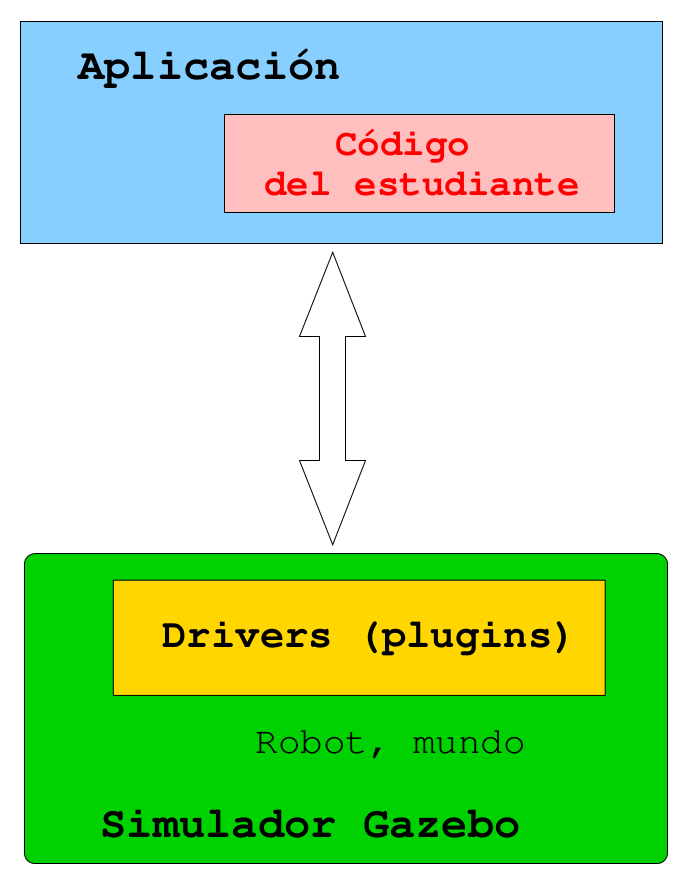
\includegraphics[width=0.8\textwidth]{esquemapracticas02.png}
			\end{figure}
		\end{center}
	\end{minipage}
\end{hslide}

\begin{hslide}
	\slsubsect{Práctica navegación local Fórmula 1.}
	\begin{itemize}
		\item Coche con sensores 
		\item Esquivar obstáculos.
		\item Algoritmo de navegación local (VFF).
	\end{itemize}
	\begin{center}
		\begin{minipage}[t]{0.55\textwidth}
			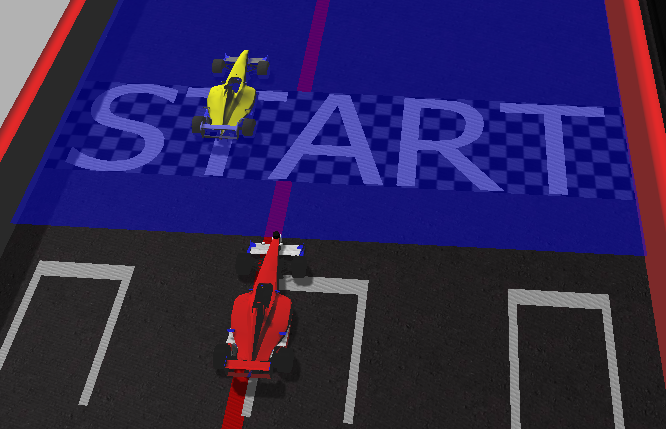
\includegraphics[width=\textwidth]{vff-gazebo.png}
		\end{minipage}
		\begin{minipage}[t]{0.25\textwidth}
			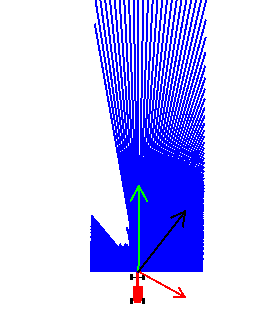
\includegraphics[width=\textwidth]{vff-gui.png}
		\end{minipage}
	\end{center}
\end{hslide}

\begin{hslide}
	\slsubsect{Práctica sigue-líneas.}
	\begin{itemize}
		\item kibuki con cámara 
		\item Seguir línea roja.
		\item Procesamiento de imágen.
	\end{itemize}
	\begin{minipage}[t]{0.47\textwidth}
		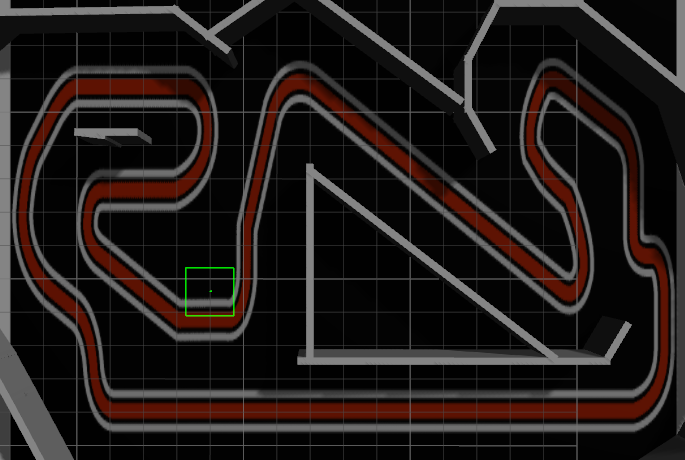
\includegraphics[width=\textwidth]{followline-world.png}
	\end{minipage}
	\begin{minipage}[t]{0.53\textwidth}
		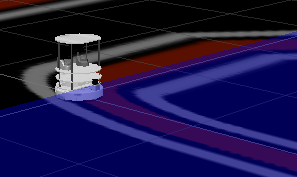
\includegraphics[width=\textwidth]{kobukiMontmelo.png}
	\end{minipage}
\end{hslide}

%%--------------------------------------------------------------
\begin{hslide}
	\slsect{Objetivo}
	Mejorar y ampliar la colección de prácticas de JdeRobot-Academy, enriqueciéndolas y aumentando el abanico de posibilidades que se ofrece al alumno.
	\begin{itemize}
		\item Mejorar la infraestructura en Gazebo de las prácticas de JdeRobot-Academy que usan coches de carreras.
		\item Diseñar y programar un teleoperador de un brazo robótico en Gazebo.
	\end{itemize}
\end{hslide}


%%--------------------------------------------------------------
\begin{hslide}
	\slsect{Infraestructura}
	\slsubsect{Blender}
	\begin{itemize}
		\item \textbf{Blender}: Programa de modelado, iluminación, renderizado, animación y creación de gráficos tridimensionales.
	\end{itemize}
	\begin{center}
		\begin{figure}
			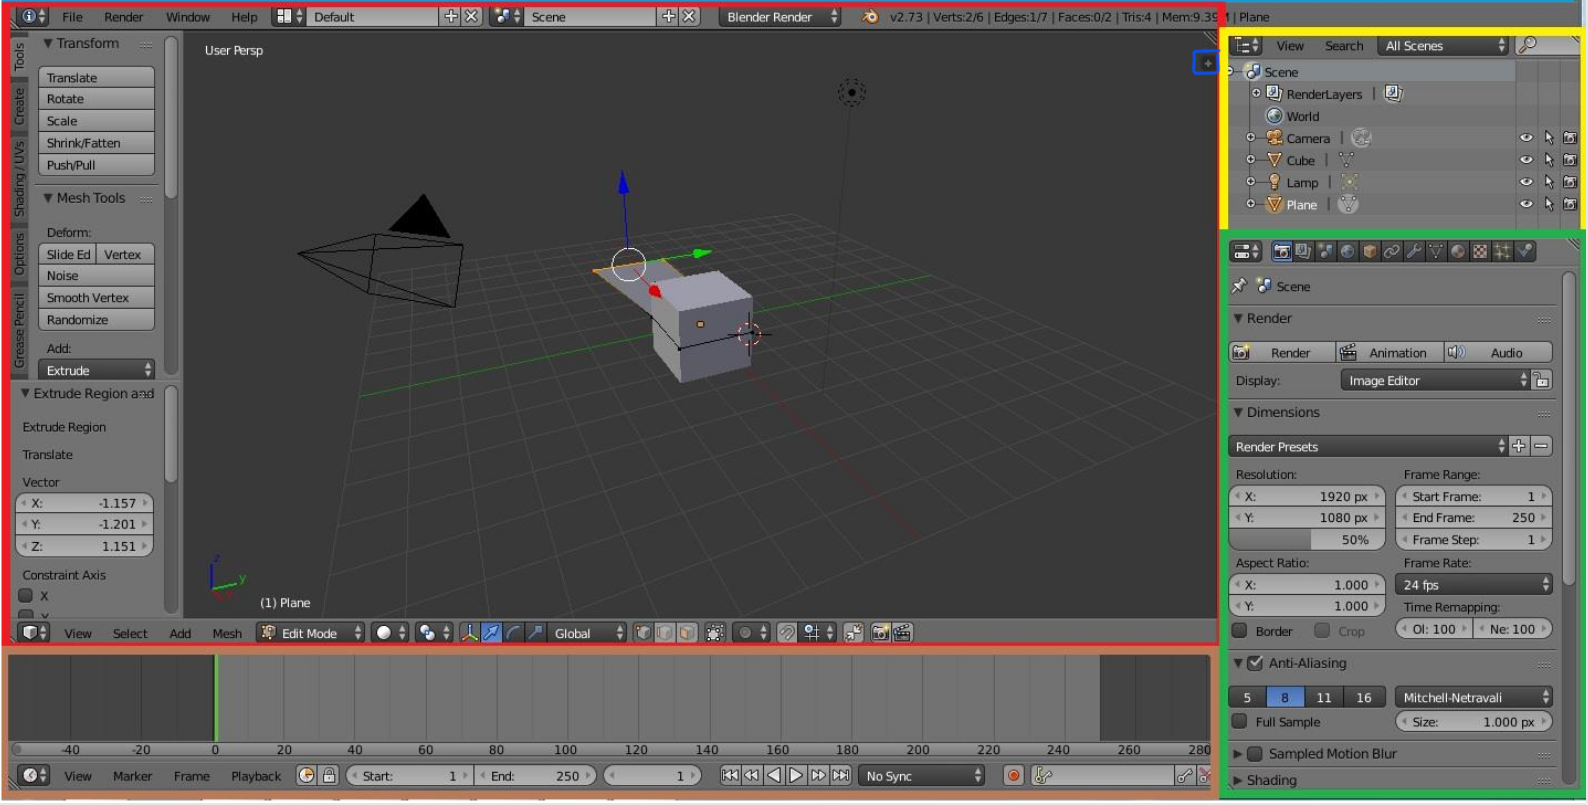
\includegraphics[width=0.8\textwidth]{InterfazBlender01.png}
		\end{figure}
	\end{center}
\end{hslide}

\begin{hslide}
	\slsubsect{Gazebo y ROS}
	\begin{itemize}
		\item \textbf{Gazebo}: Simula sensores, actuadores, robots,... en mundos virtuales.
		\item \textbf{ROS}: Es un \textit{middleware} para robots.
	\end{itemize}
	\begin{center}
		\begin{figure}
			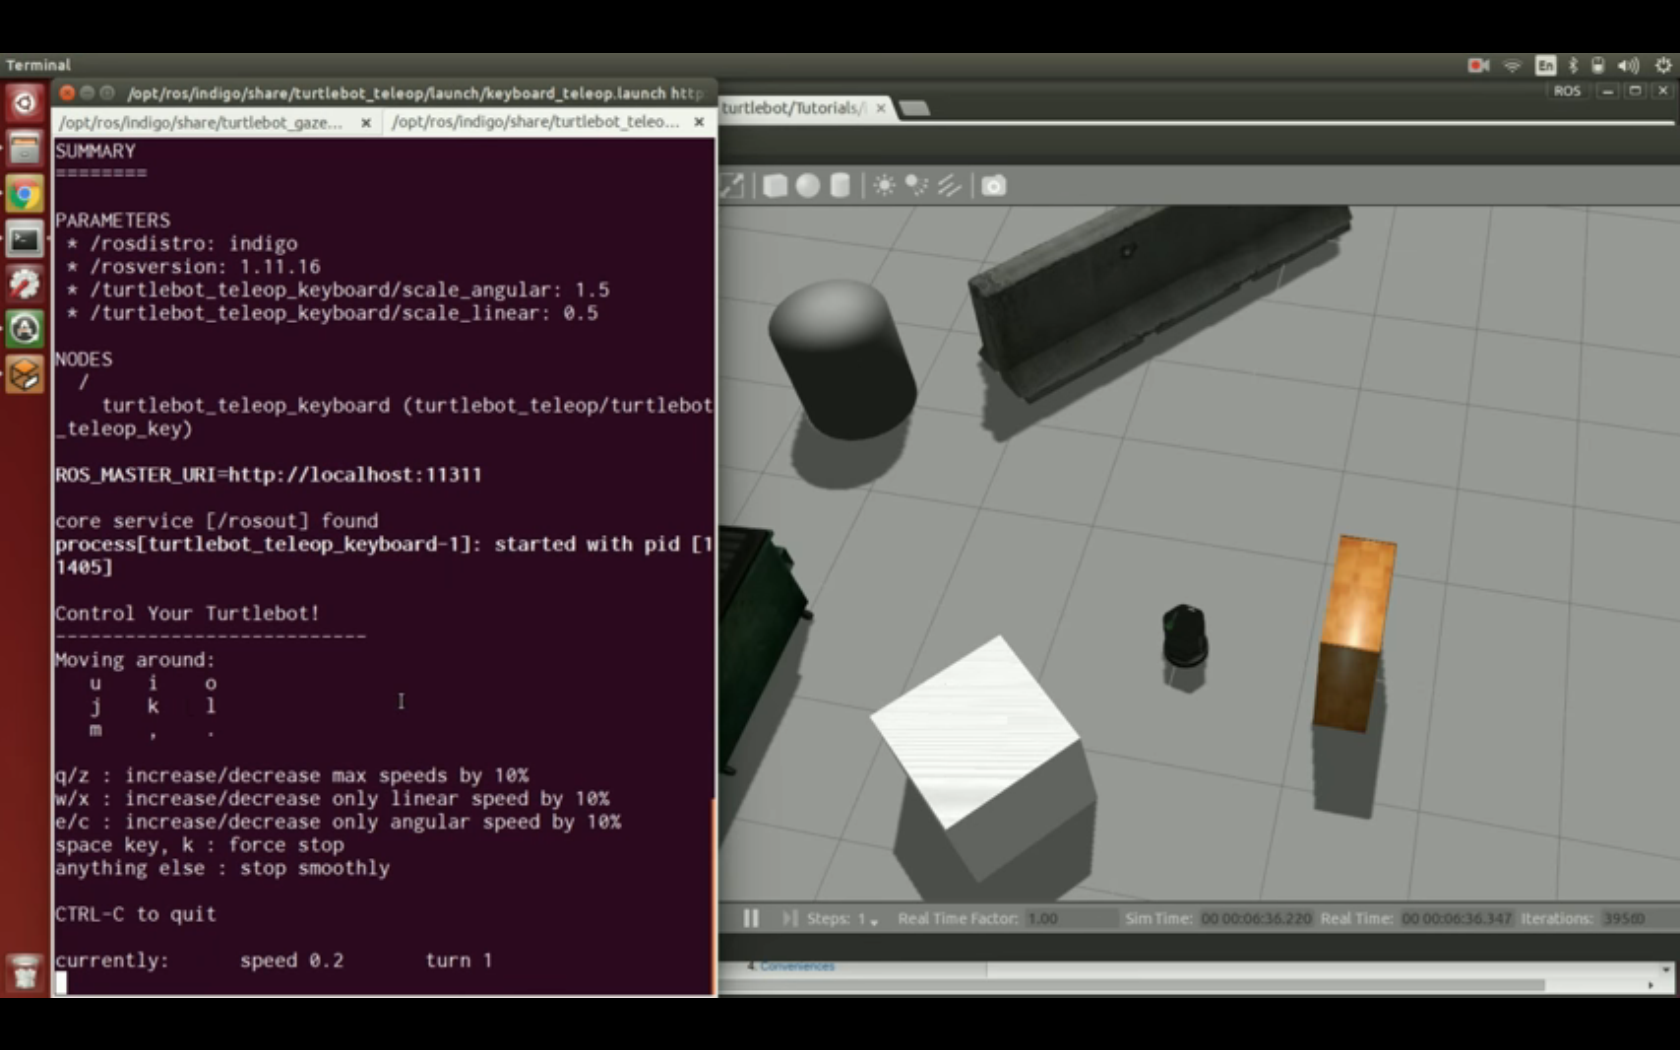
\includegraphics[width=0.7\textwidth]{ros.png}
		\end{figure}
	\end{center}
\end{hslide}

\begin{hslide}
	\slsubsect{ARIAC}
	\begin{center}(Agile Robotics for Industrial Automation Competition). \end{center}
	Competición para probar la agilidad de los sistemas robóticos industriales.
	\begin{center}
		\begin{figure}
			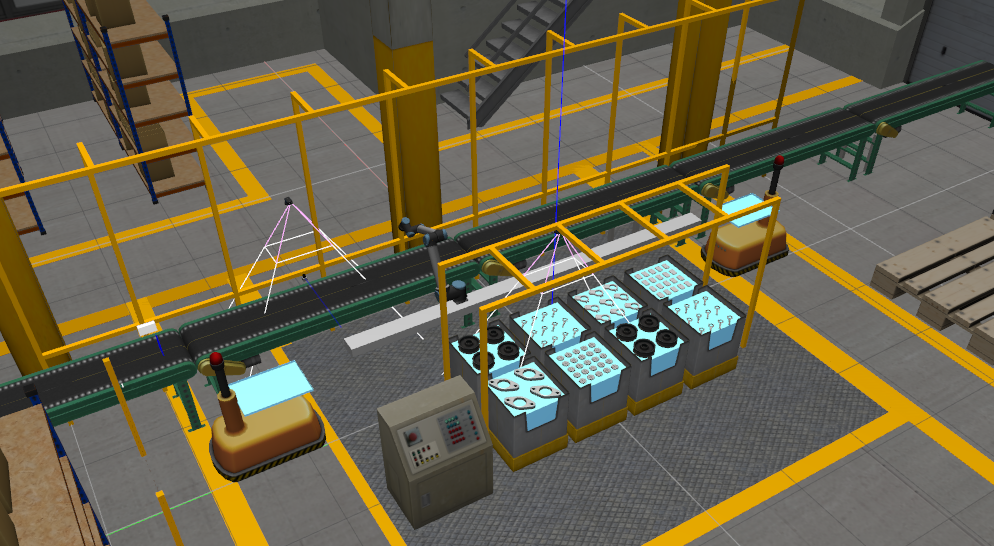
\includegraphics[width=0.7\textwidth]{ariac01.png}
		\end{figure}
	\end{center}
\end{hslide}


%%--------------------------------------------------------------
\begin{hslide}
	\slsect{Circuito de carreras de Fórmula 1}
	\begin{itemize}
		\item Reconstruir el circuito de Mónaco de forma que se pueda utilizar en:
		\begin{itemize}
			\item Práctica sigue línea.
			\item Práctica navegación local.
		\end{itemize}
		\item Creación de mundos para Gazebo que sigan el esquema de las practicas.
	\end{itemize}
\end{hslide}

\begin{hslide}
	\slsubsect{Esquema de componentes}
	\begin{center}
		\begin{figure}
			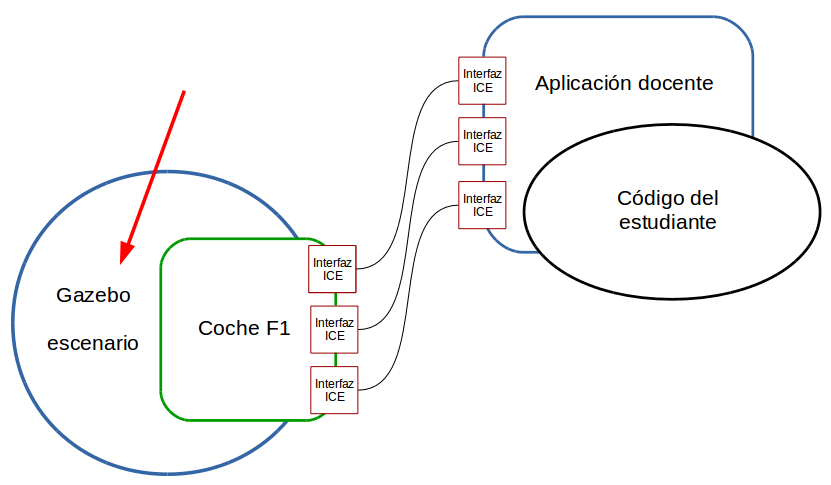
\includegraphics[width=\textwidth]{graficof1.png}
		\end{figure}
	\end{center}
\end{hslide}


\begin{hslide}
	\slsubsect{Circuito plano}
	\begin{minipage}{0.45\textwidth}
		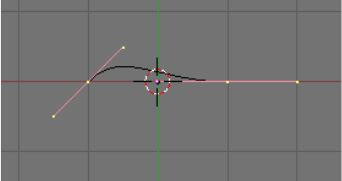
\includegraphics[width=\textwidth]{InterfazBlender05.png}
		\begin{center}
			Curva Bezier
		\end{center}
	\end{minipage}
	\begin{minipage}{0.1\textwidth}
		\begin{center}
			
\includegraphics[width=0.5\textwidth]{mas.jpg}
		\end{center}
	\end{minipage}
	\begin{minipage}{0.5\textwidth}
		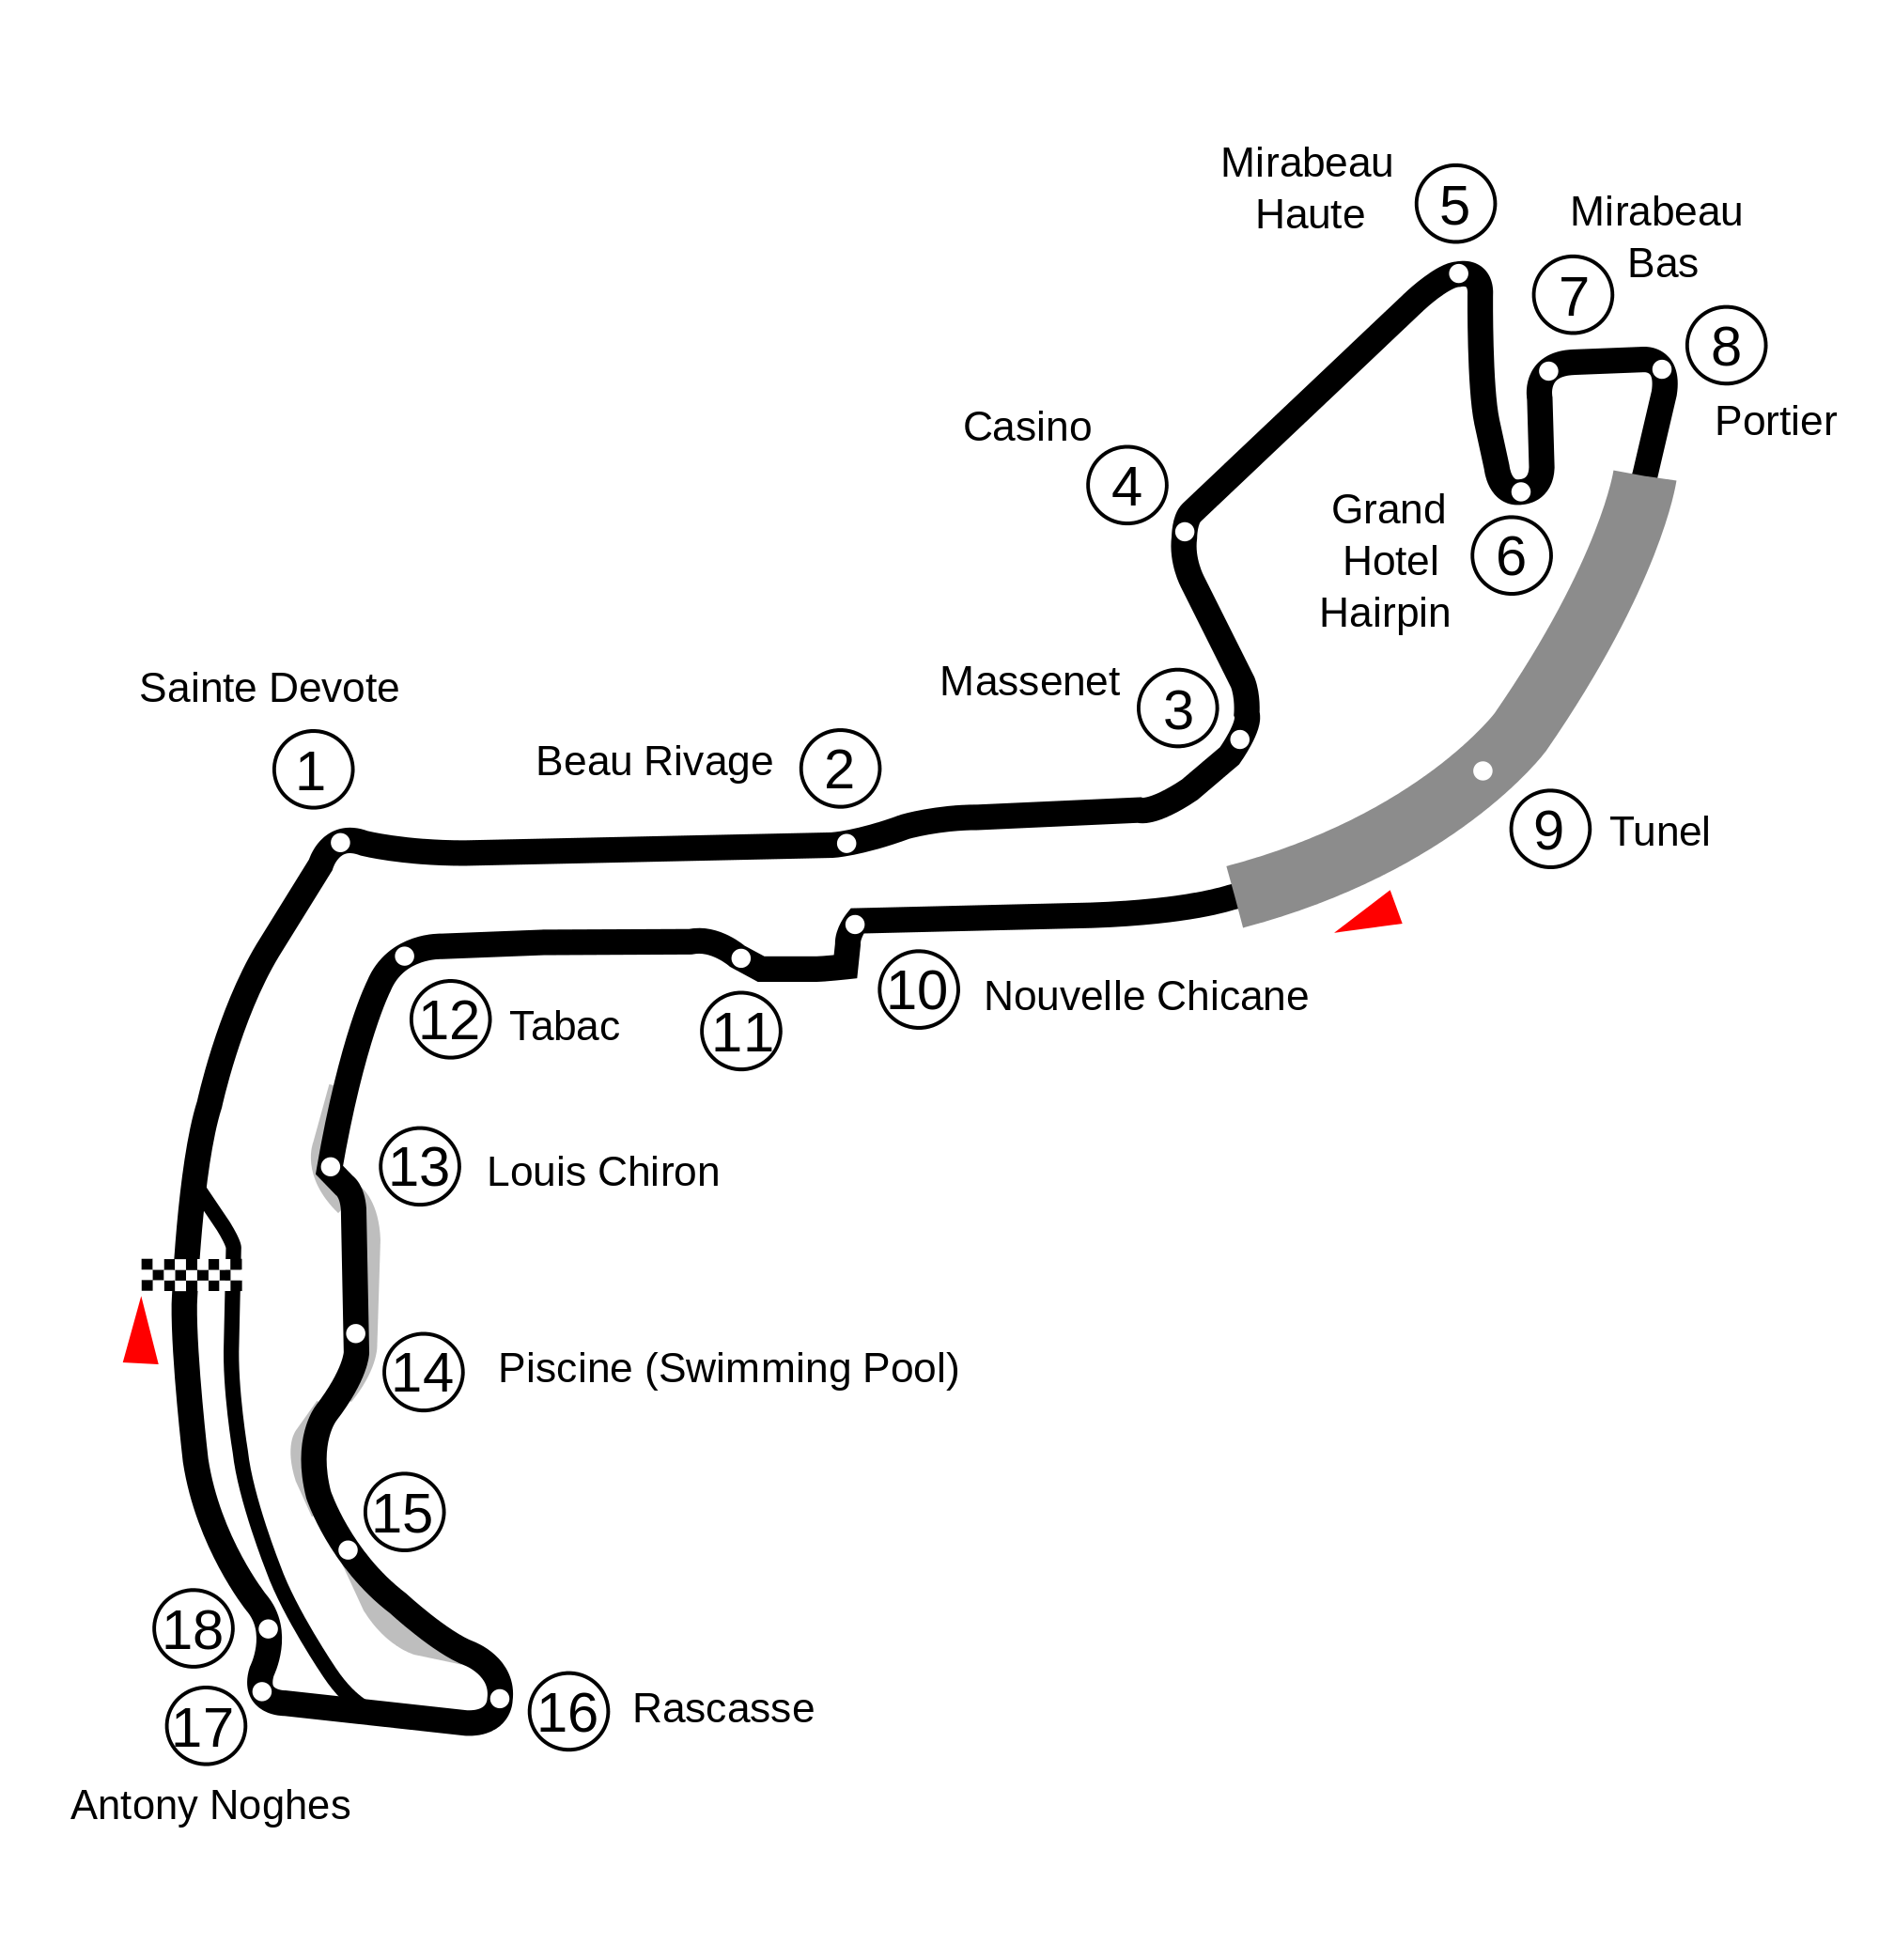
\includegraphics[width=\textwidth]{CircuitoMonaco.png}
		\begin{center}
			Plano del circuito
		\end{center}
	\end{minipage}
\end{hslide}


\begin{hslide}
	\begin{center}
		\begin{figure}
			\begin{center}
				Curva del trazado
			\end{center}
			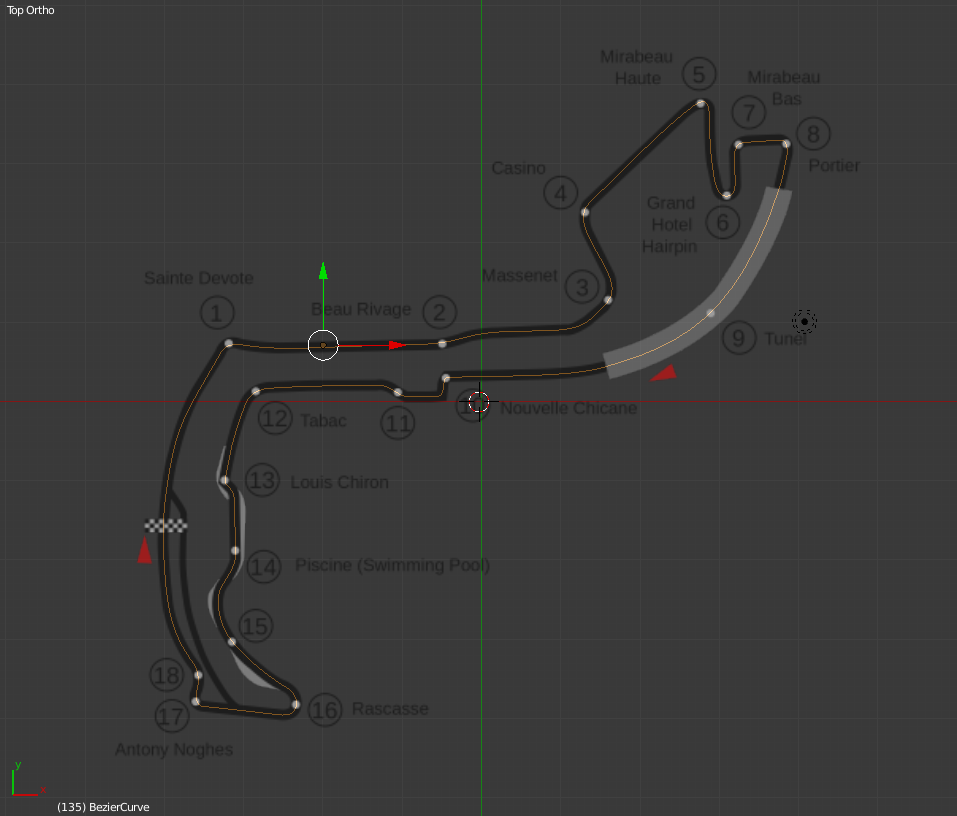
\includegraphics[width=0.75\textwidth]{MonacoTrazado.png}
		\end{figure}
	\end{center}
\end{hslide}

\begin{hslide}
	\begin{itemize}
	\item Modelamos un segmento de circuito. Creamos:
	\begin{itemize}
		\item Carretera.
		\item Vallas.
		\item Aceras.
	\end{itemize}
	\item Texturizamos cada zona.
	\item Asignamos materiales a las superficies.
\end{itemize}
\end{hslide}

\begin{hslide}
	\begin{center}
		\begin{figure}
			\begin{center}
				Segmento del circuito
			\end{center}
			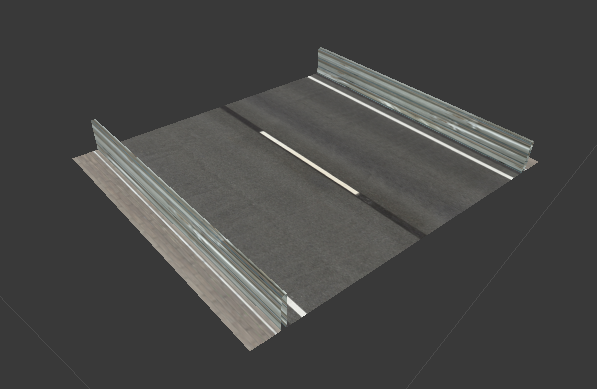
\includegraphics[width=0.82\textwidth]{MonacoSegmento.png}
		\end{figure}
	\end{center}
\end{hslide}

\begin{hslide}
	\begin{center}
		Aplicamos modificadores:
	\end{center}
	\begin{minipage}{0.45\textwidth}
		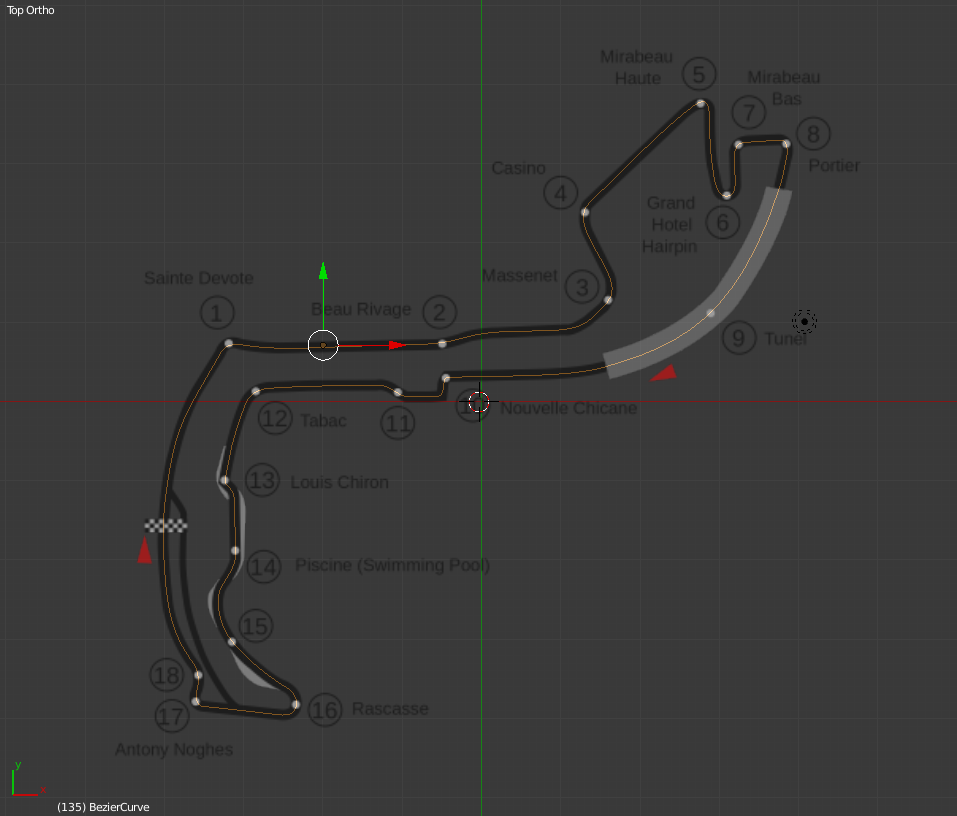
\includegraphics[width=\textwidth]{MonacoTrazado.png}
	\end{minipage}
	\begin{minipage}{0.1\textwidth}
		\begin{center}
			
\includegraphics[width=0.5\textwidth]{mas.jpg}
		\end{center}
	\end{minipage}
	\begin{minipage}{0.45\textwidth}
		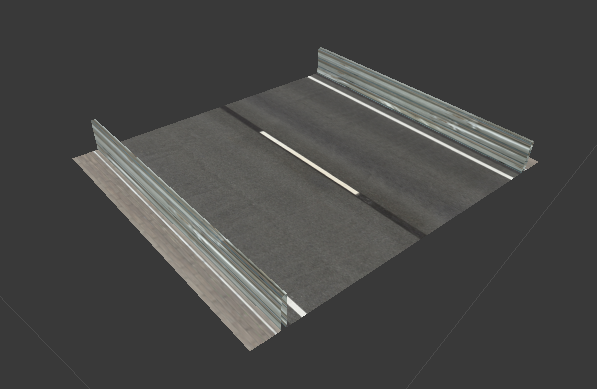
\includegraphics[width=\textwidth]{MonacoSegmento.png}
	\end{minipage}
\end{hslide}

\begin{hslide}
	\begin{center}
		Circuito modelado:
		\begin{figure}
			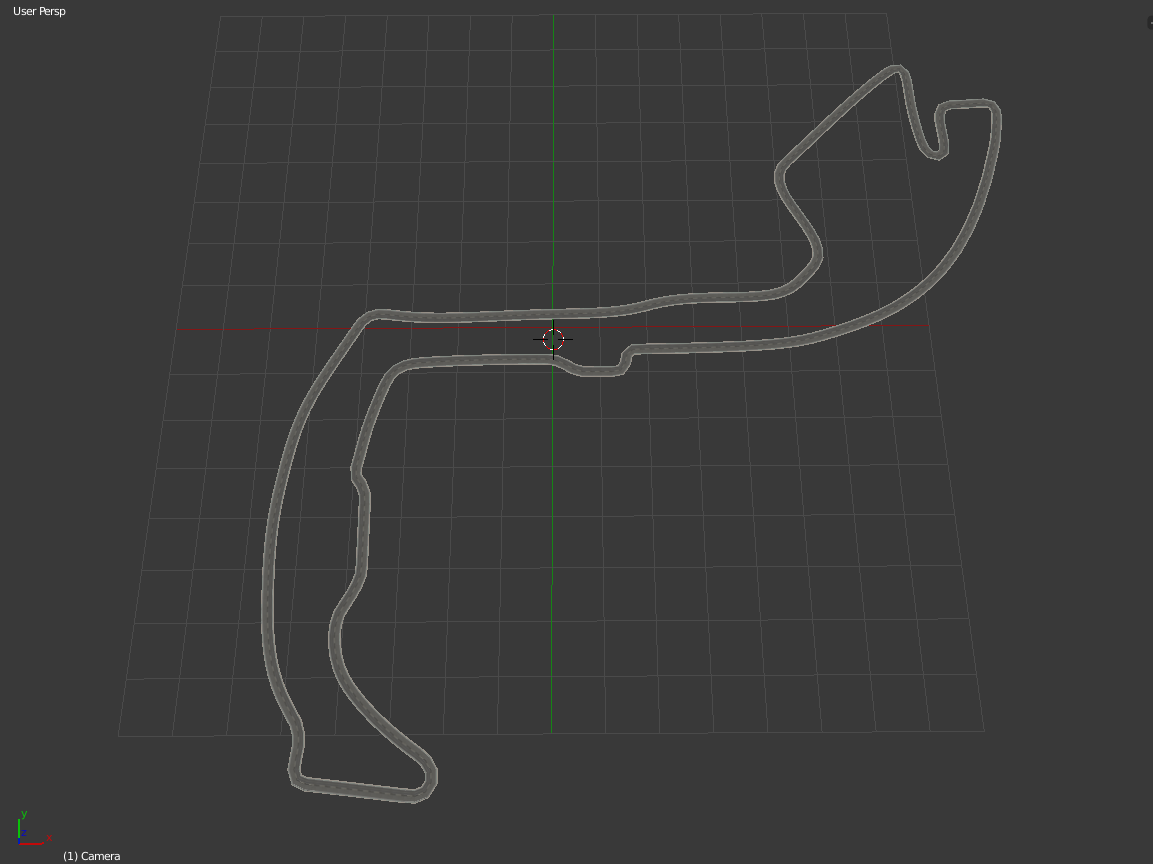
\includegraphics[width=0.82\textwidth]{Circuito00.png}
		\end{figure}
	\end{center}
\end{hslide}

\begin{hslide}
	\begin{center}
		Detalle del circuito modelado:
		\begin{figure}
			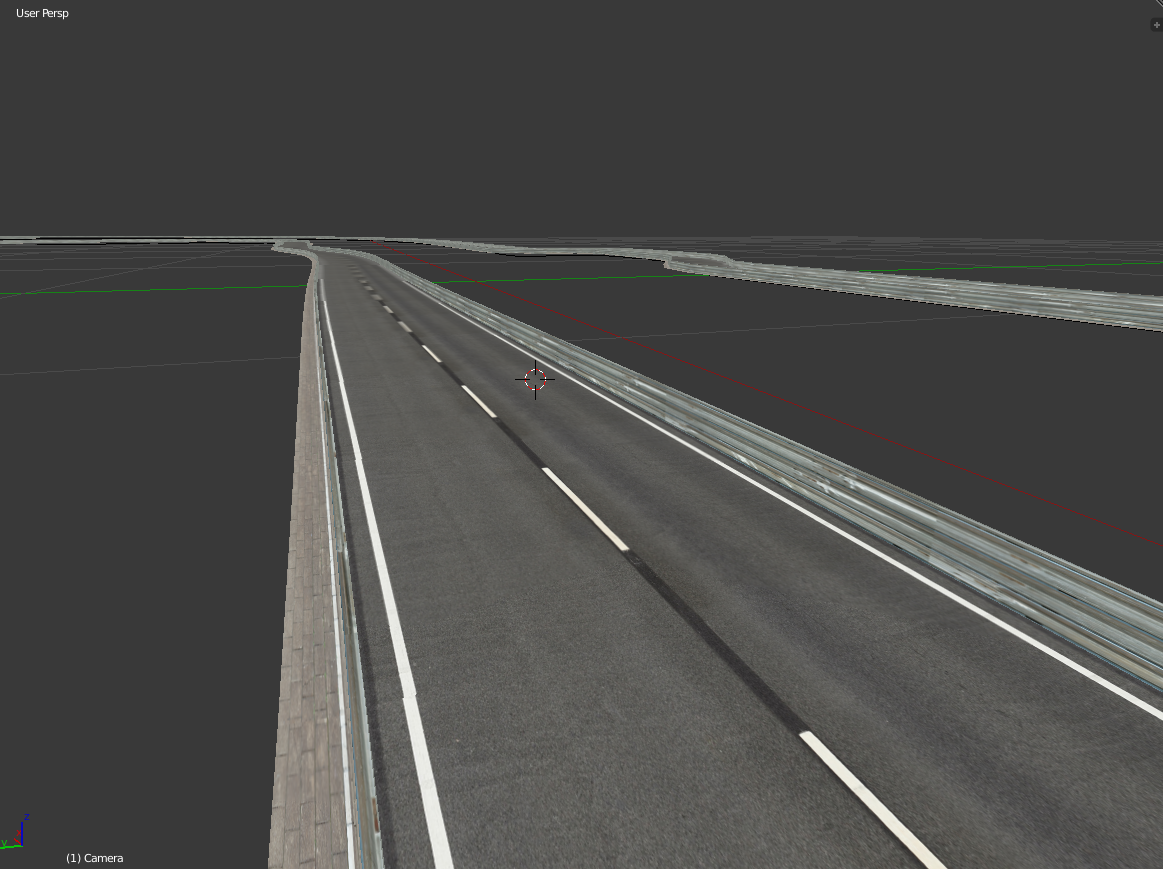
\includegraphics[width=0.82\textwidth]{Circuito01.png}
		\end{figure}
	\end{center}
\end{hslide}

\begin{hslide}
	\begin{minipage}{0.5\textwidth}
		\begin{itemize}
			\item Añadimos fondo al circuito
			\item Texturizamos de forma realista
		\end{itemize}
	\end{minipage}
	\begin{minipage}{0.5\textwidth}
		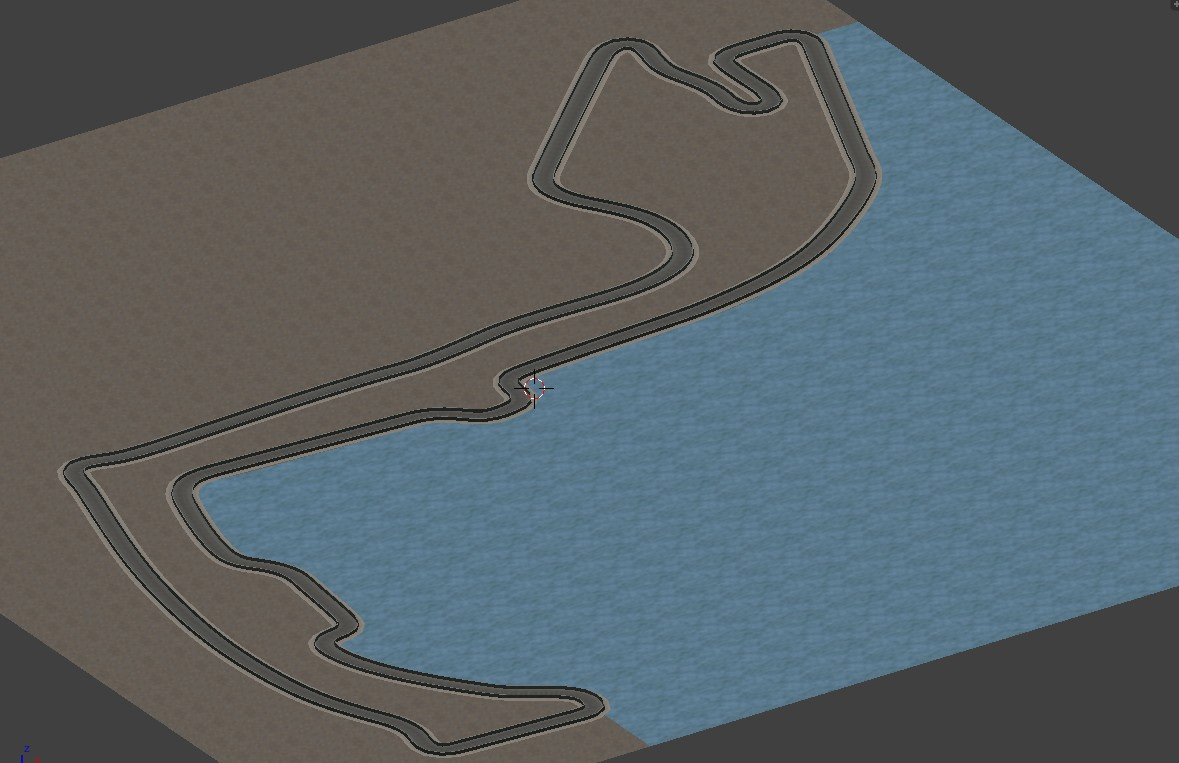
\includegraphics[width=\textwidth]{MonacoPlano1.jpg}
	\end{minipage}
\end{hslide}

\begin{hslide}
	\begin{minipage}{0.5\textwidth}
		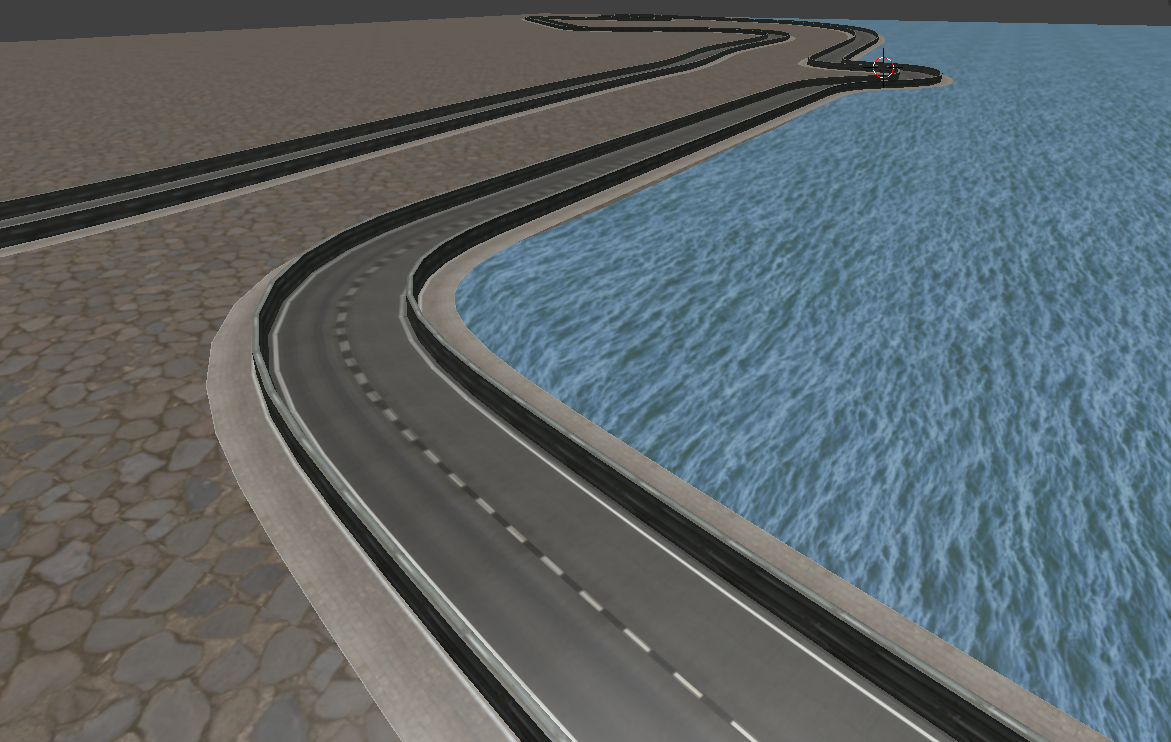
\includegraphics[width=\textwidth]{MonacoPlano3.png}
	\end{minipage}
	\begin{minipage}{0.515\textwidth}
		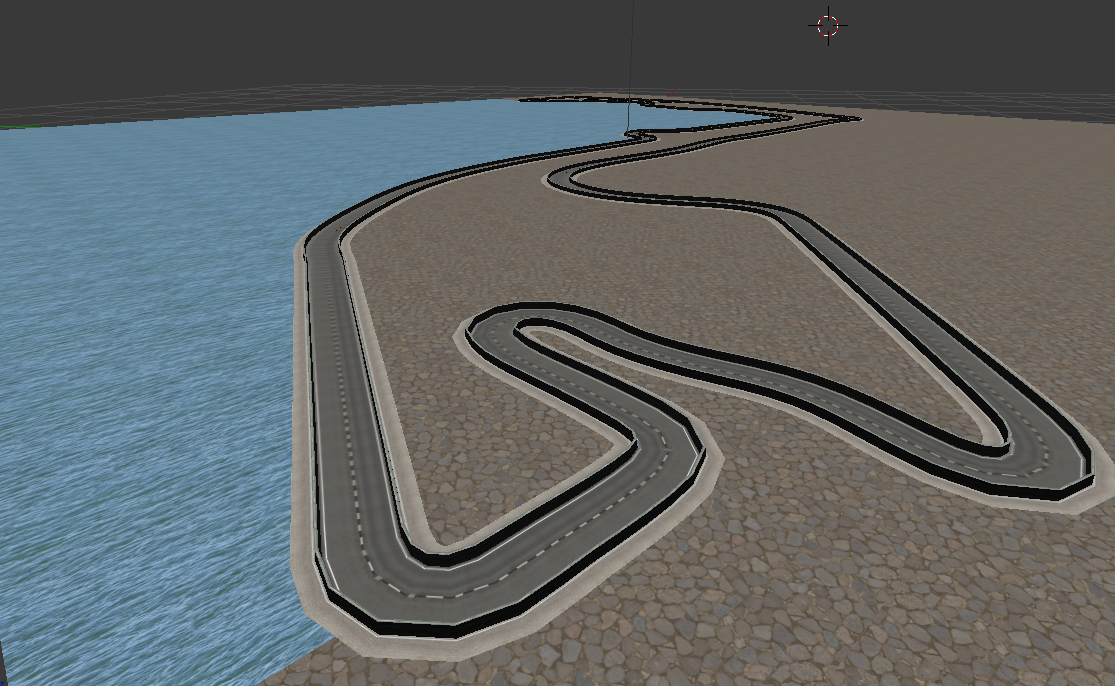
\includegraphics[width=\textwidth]{MonacoPlano9.png}
	\end{minipage}
	\begin{minipage}{0.5\textwidth}
		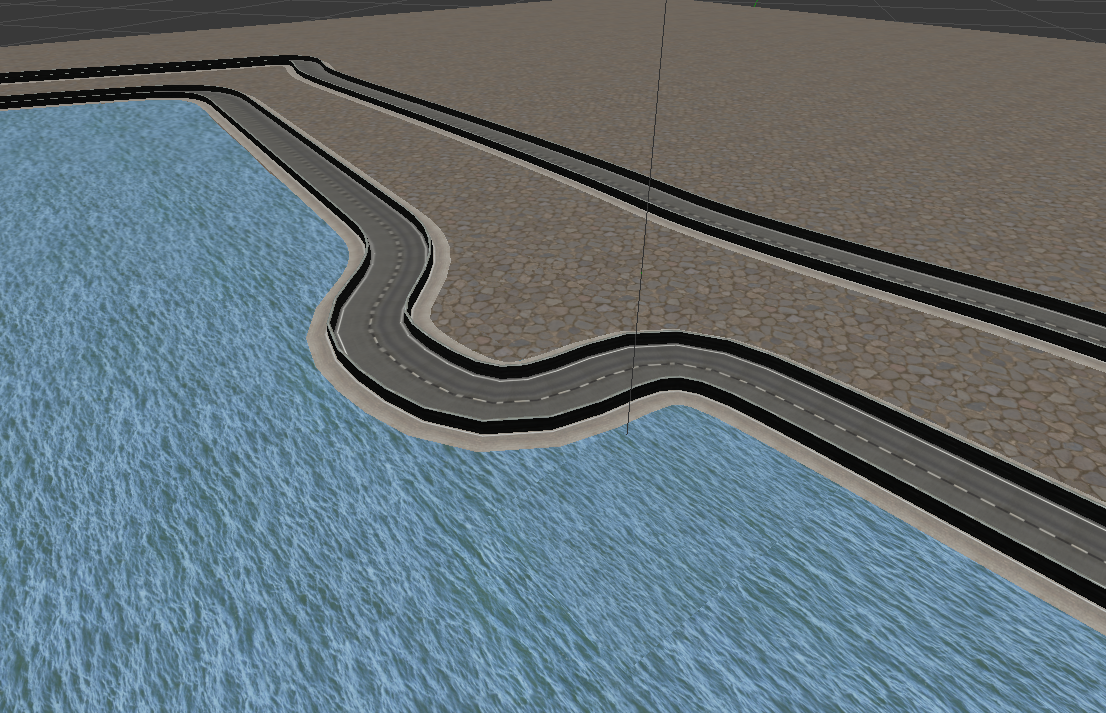
\includegraphics[width=\textwidth]{MonacoPlano10.png}
	\end{minipage}
	\begin{minipage}{0.53\textwidth}
		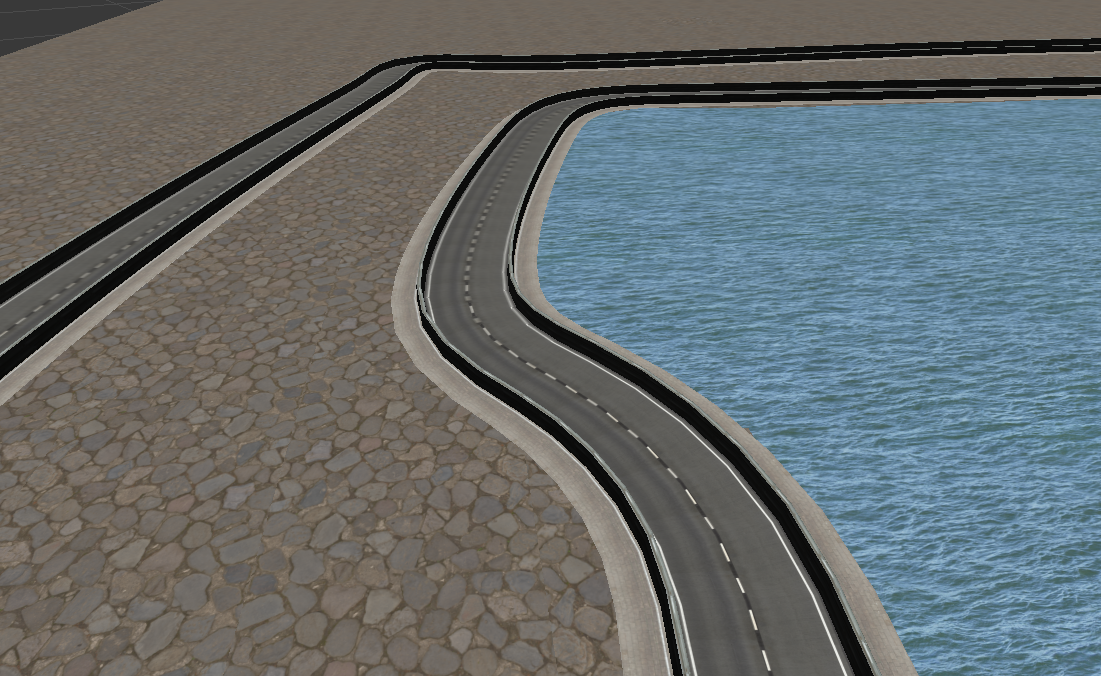
\includegraphics[width=\textwidth]{MonacoPlano2.png}
	\end{minipage}
\end{hslide}

\begin{hslide}
	\slsubsect{Circuito con elevaciones}
	\begin{itemize}
		\item Creamos \textit{mesh} y esculpimos el fondo.
		\item Modelamos y texturizamos trazado.
		\item “Modificamos” el trazado con \textit{mesh}.
		\item Texturizamos el circuito.
	\end{itemize}
	\begin{center}
		\begin{figure}
			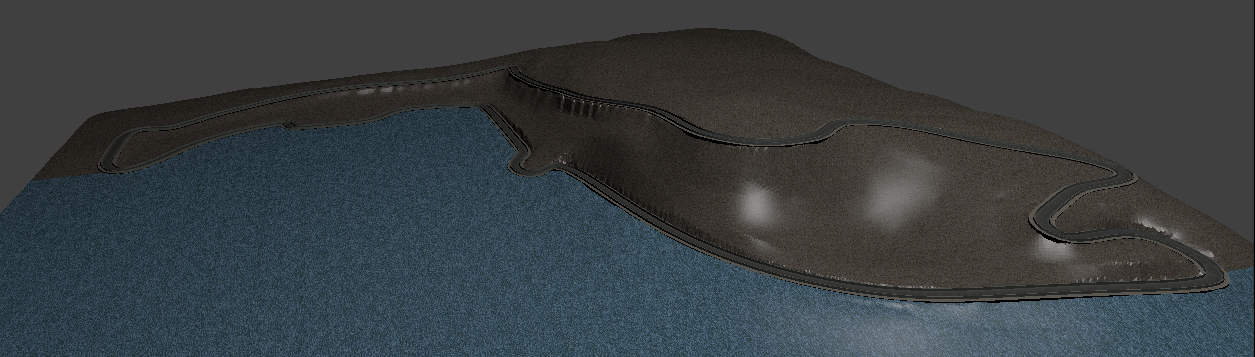
\includegraphics[width=\textwidth]{MonacoElev05.png}
		\end{figure}
	\end{center}
\end{hslide}

\begin{hslide}
	\begin{minipage}{0.5\textwidth}
		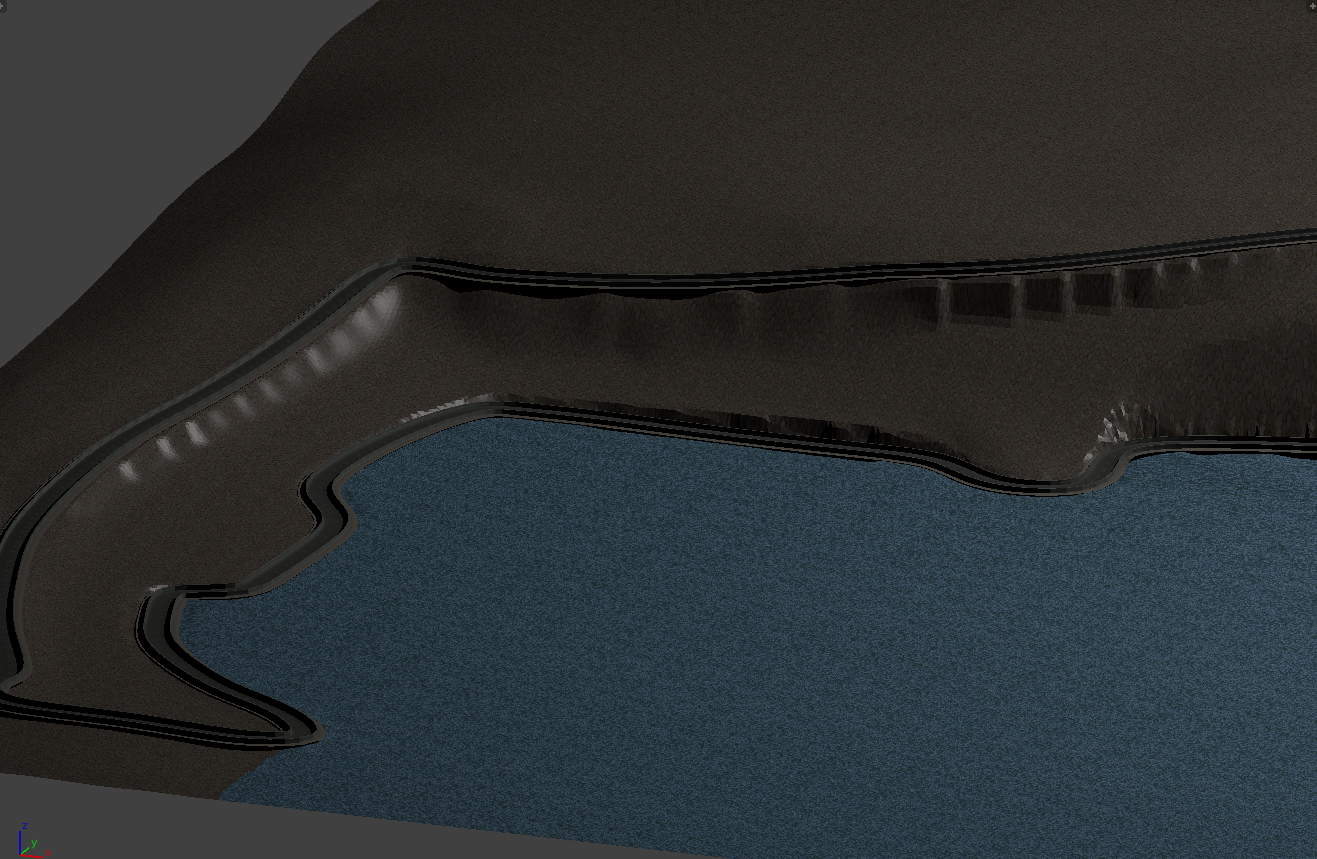
\includegraphics[width=\textwidth]{MonacoElev01.png}
	\end{minipage}
	\begin{minipage}{0.5\textwidth}
		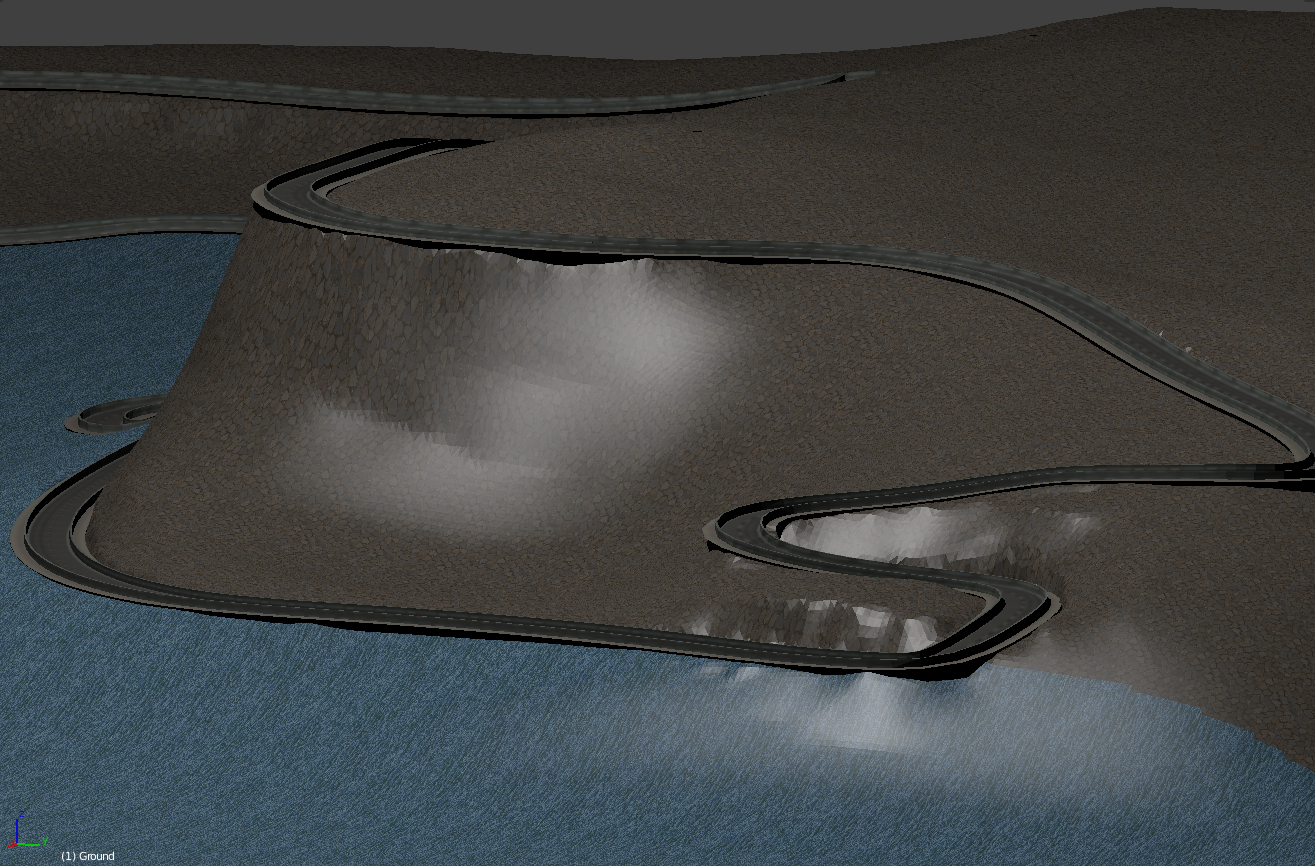
\includegraphics[width=\textwidth]{MonacoElev02.png}
	\end{minipage}
	\begin{minipage}{0.5\textwidth}
		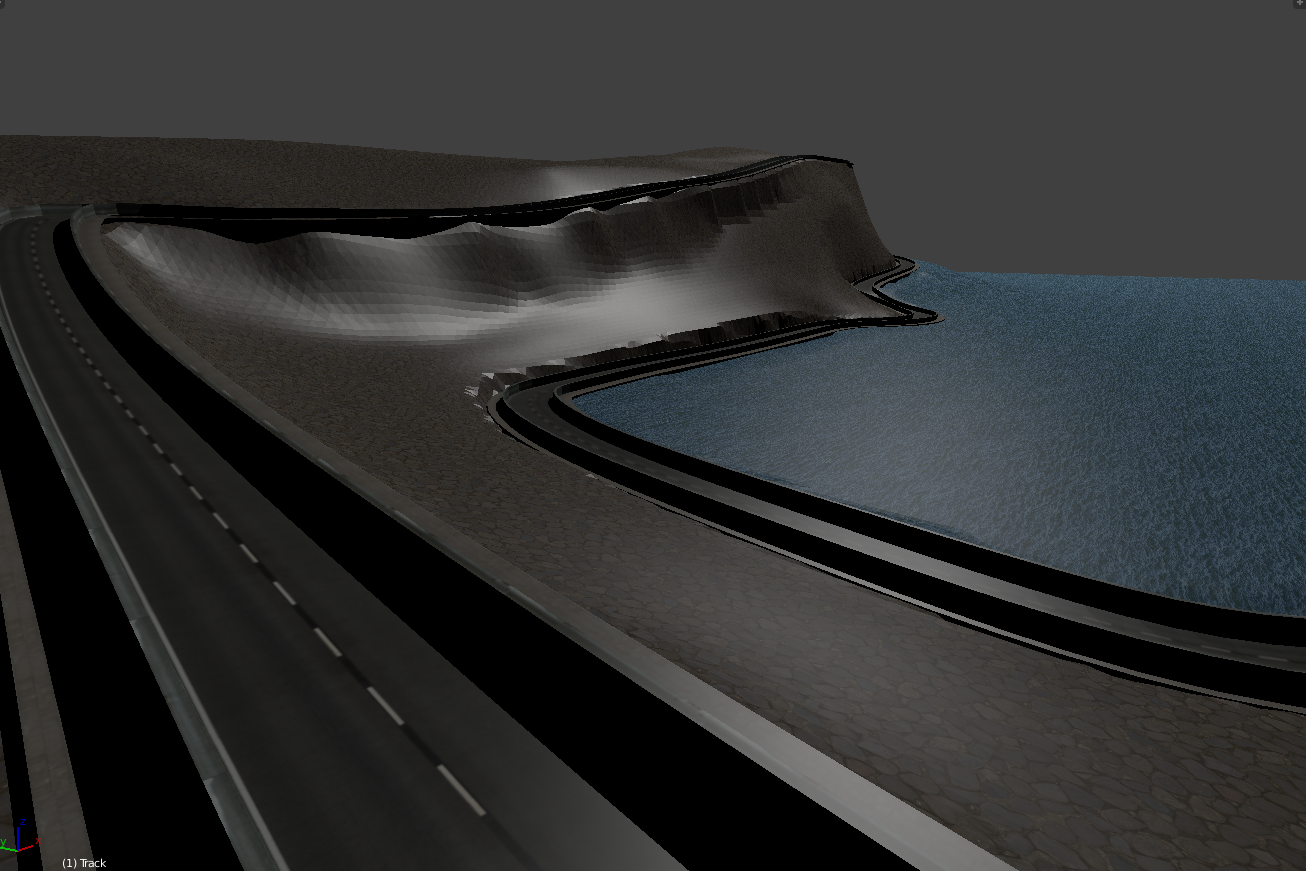
\includegraphics[width=\textwidth]{MonacoElev03.png}
	\end{minipage}
	\begin{minipage}{0.51\textwidth}
		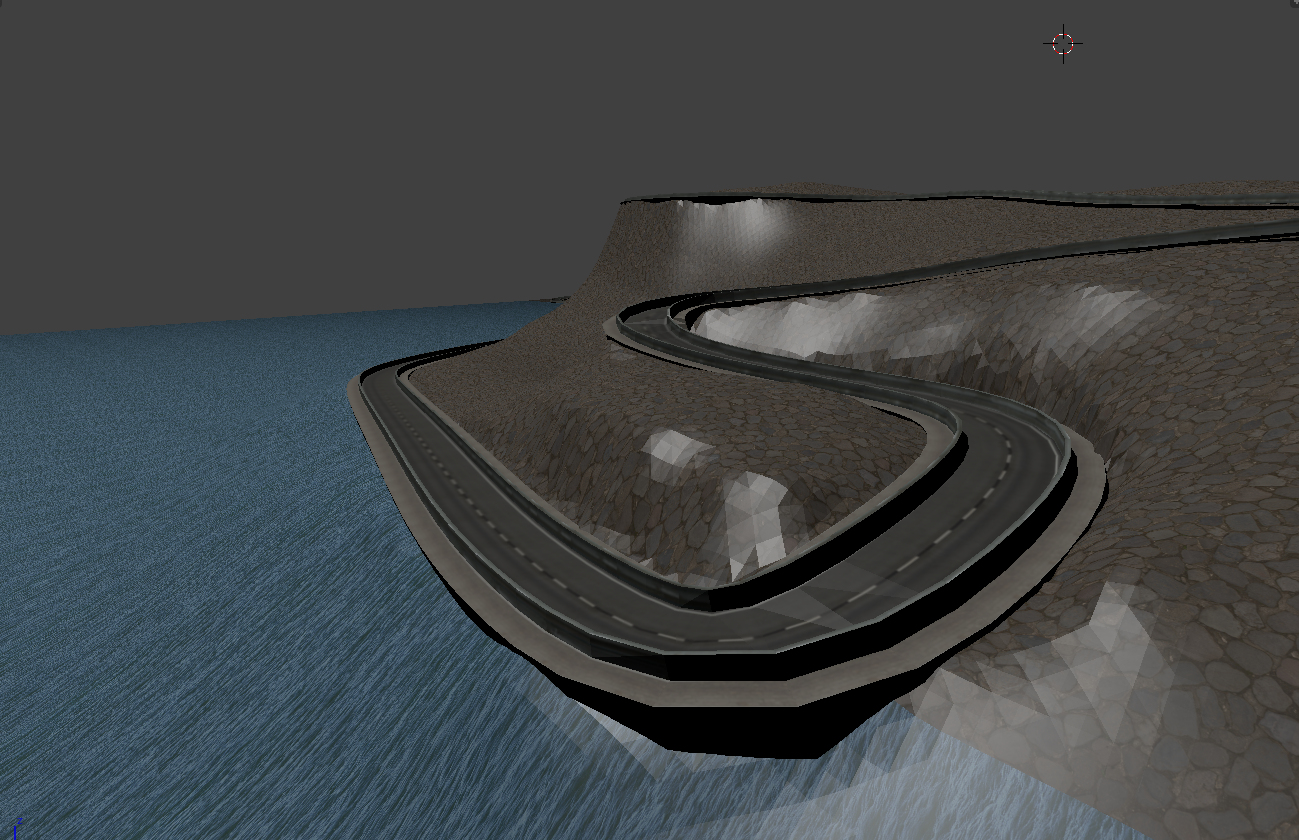
\includegraphics[width=\textwidth]{MonacoElev04.png}
	\end{minipage}
\end{hslide}

\begin{hslide}
	\slsubsect{Circuitos con línea roja}
	Modificamos la textura del asfalto pintando la línea roja.
	
	\begin{minipage}{0.5\textwidth}
		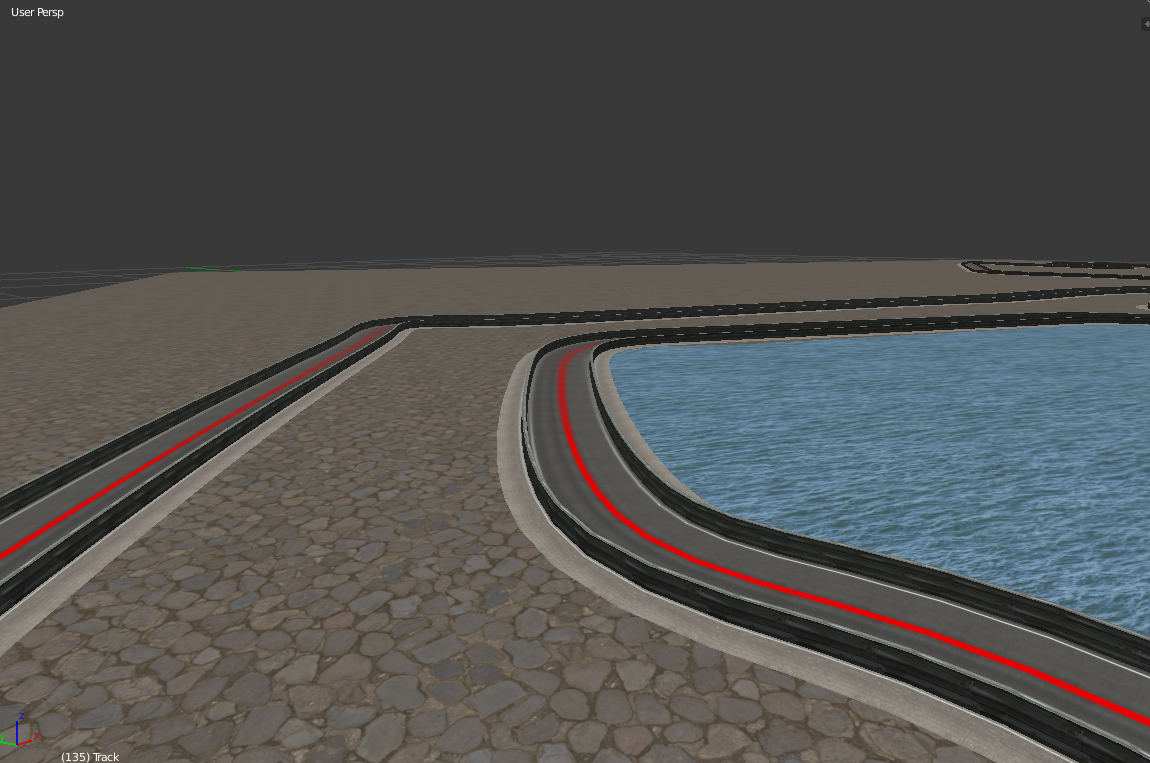
\includegraphics[width=\textwidth]{monacolinea.png}
	\end{minipage}
	\begin{minipage}{0.51\textwidth}
		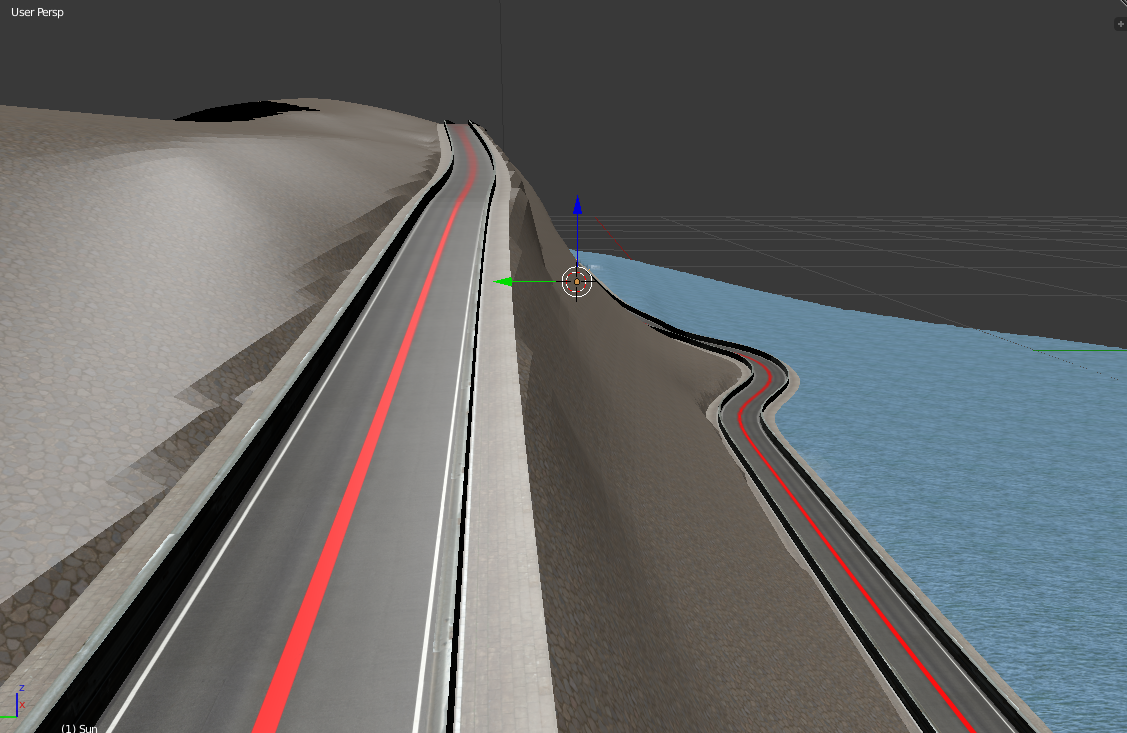
\includegraphics[width=\textwidth]{monacoelevlinea.png}
	\end{minipage}
\end{hslide}

\begin{hslide}
	\slsubsect{Circuitos en las prácticas}
	\begin{minipage}{0.5\textwidth}
		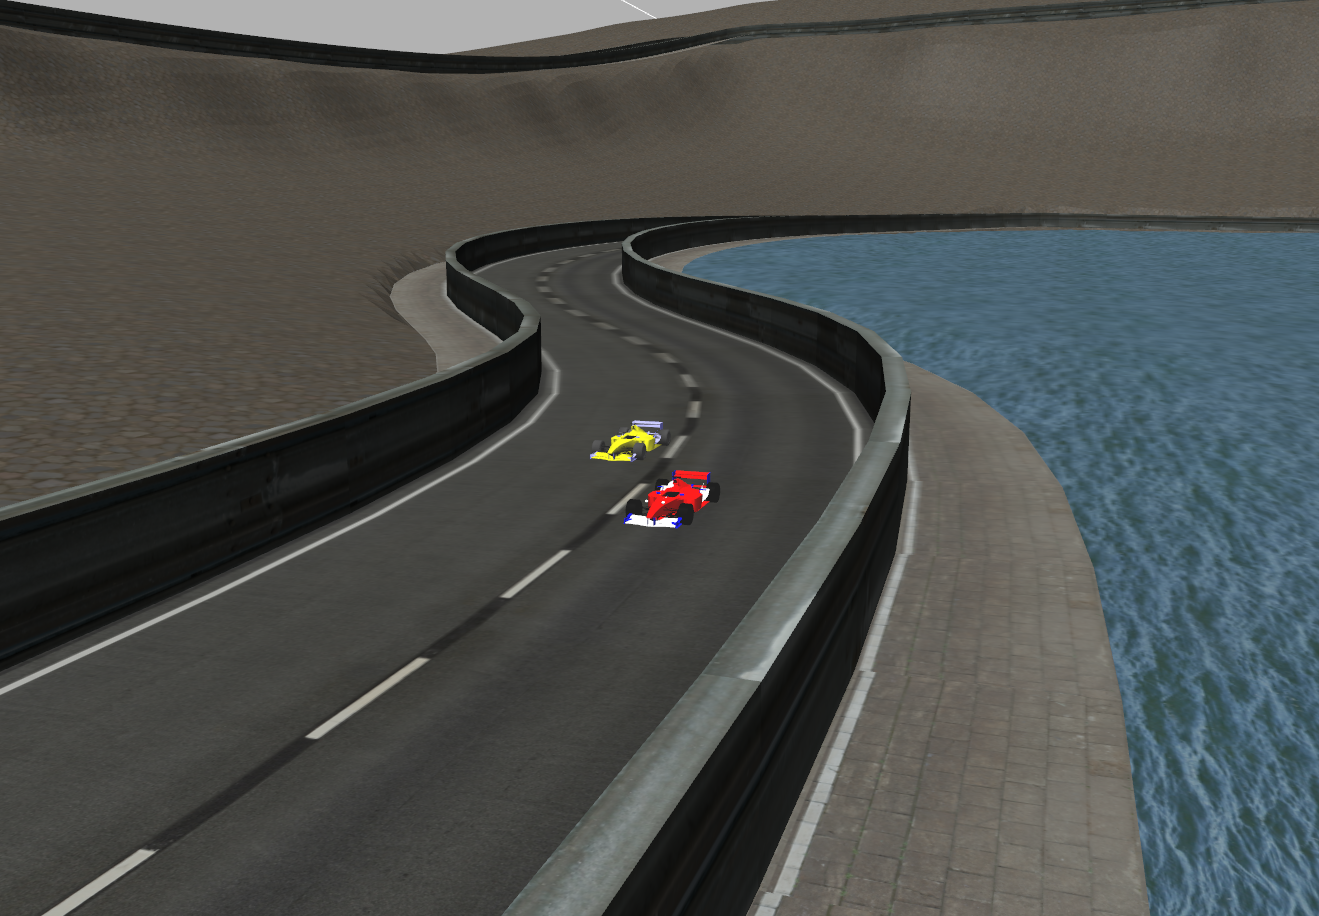
\includegraphics[width=\textwidth]{MonacoElev07.png}
	\end{minipage}
	\begin{minipage}{0.5\textwidth}
		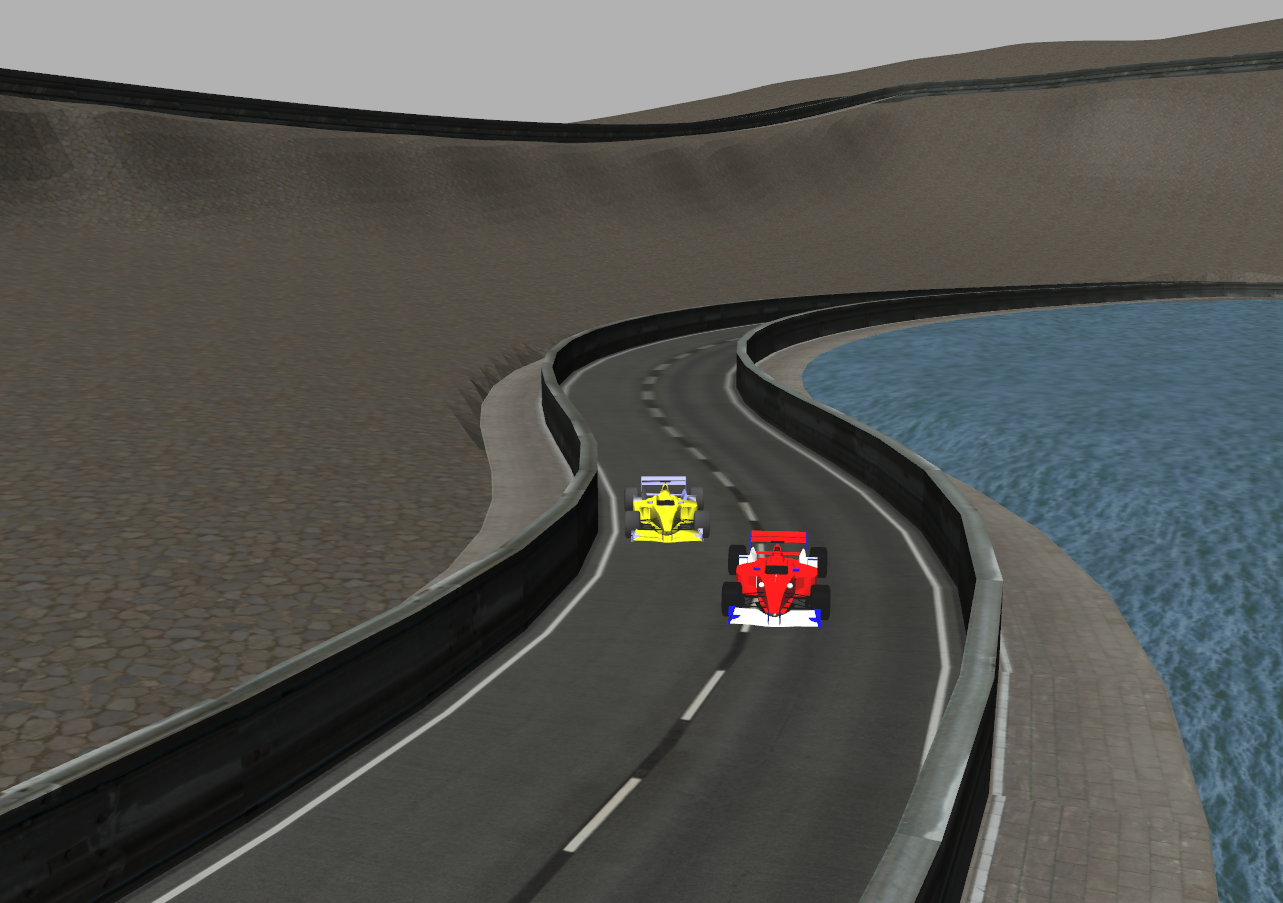
\includegraphics[width=\textwidth]{MonacoElev08.png}
	\end{minipage}
\end{hslide}




%%--------------------------------------------------------------
\begin{hslide}
	\slsect{Brazo robótico}
	\begin{minipage}{0.6\textwidth}
		\begin{itemize}
			\item Buscamos brazo que reuna requisitos:
			\begin{itemize}
				\item Gazebo 7.
				\item ROS Kinetic.
			\end{itemize}
			\item Elegimos escenario ARIAC:
			\begin{itemize}
				\item UR10
			\end{itemize}
		\end{itemize}
	\end{minipage}
	\begin{minipage}{0.4\textwidth}
		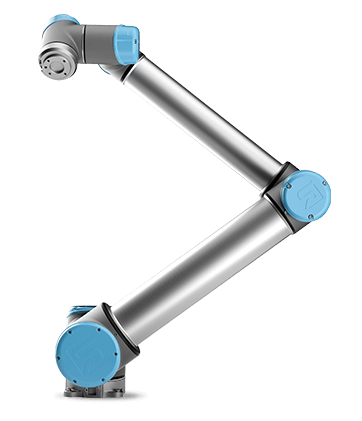
\includegraphics[width=\textwidth]{ur10.png}
	\end{minipage}
\end{hslide}

\begin{hslide}
	\slsubsect{Esquema de componentes}
	\begin{center}
		\begin{figure}
			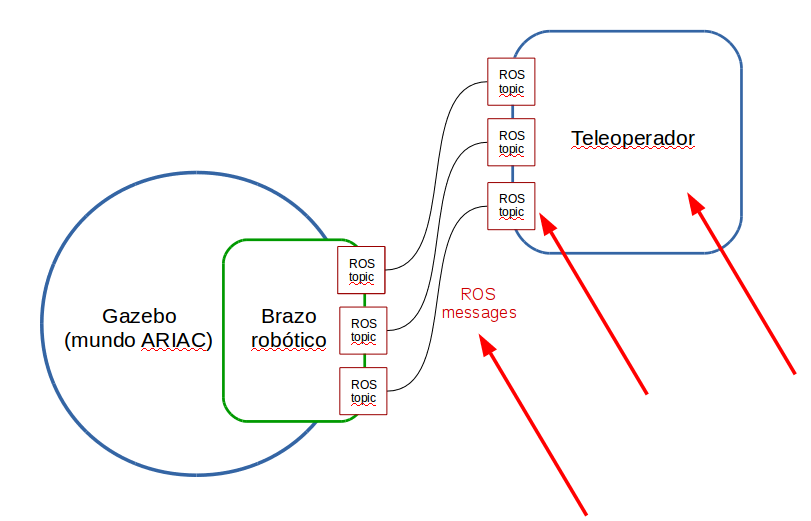
\includegraphics[width=0.95\textwidth]{graficobrazo.png}
		\end{figure}
	\end{center}
\end{hslide}

\begin{hslide}
	\slsubsect{ROS}
	Elementos básicos:
	\begin{itemize}
		\item \textbf{Nodos}: Procesos ejecutables. Se comunican entre sí:
		\begin{itemize}
			\item \textbf{}: Publica en topics.
			\item \textit{Subscriber}: Recibe de topics.
		\end{itemize}
		\item \textbf{\textit{Topics}}: Canales de comunicación entre nodos de tipado fuerte. 
		\item \textbf{Mensajes}: Estructuras de datos que se envían por los topics.
	\end{itemize}
	Se organiza en grafo.
\end{hslide}


\begin{hslide}
	\slsubsect{ARIAC en ROS}
	\begin{center}
		\begin{figure}
			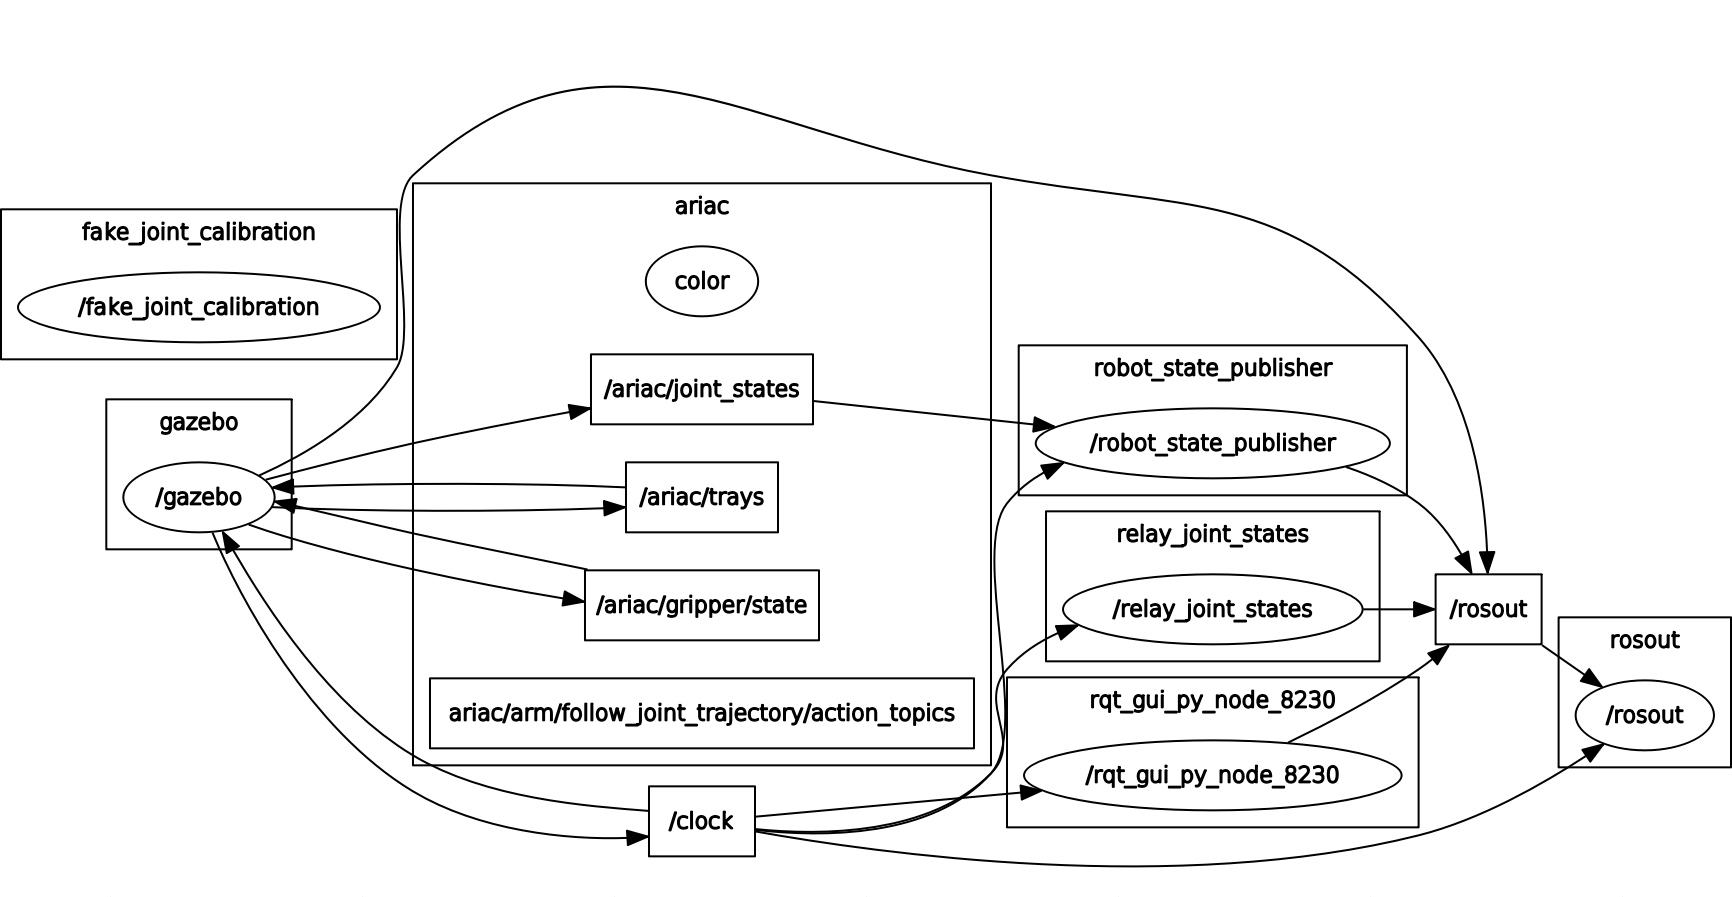
\includegraphics[width=\textwidth]{Brazo10.png}
		\end{figure}
	\end{center}
\end{hslide}

\begin{hslide}
	\slsubsect{\textit{Topics} y mensajes importantes}
\begin{itemize}
	\item \textbf{/ariac/joint\_states}: Publica las posiciones de las articulaciones del brazo.
	\begin{itemize}
		\item Mensaje: \textit{sensor\_msgs/JointState Message}.
	\end{itemize}
	\item \textbf{/ariac/arm/command}: Recibe la posición a la que mover el brazo.
	\begin{itemize}
		\item Mensaje: \textit{trajectory\_msgs/JointTrajectory Message}.
	\end{itemize}
\end{itemize}
\end{hslide}

\begin{hslide}
	\slsubsect{Articulaciones del brazo}
	\begin{center}
		\begin{figure}
			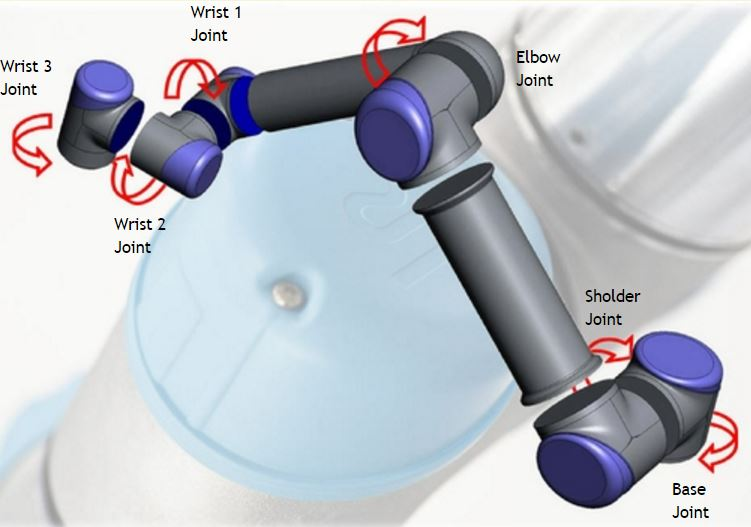
\includegraphics[width=0.8\textwidth]{brazoarticulaciones.jpg}
		\end{figure}
	\end{center}
\end{hslide}

\begin{hslide}
	\slsubsect{Mensaje de posición}
	\begin{center}
		\begin{figure}
			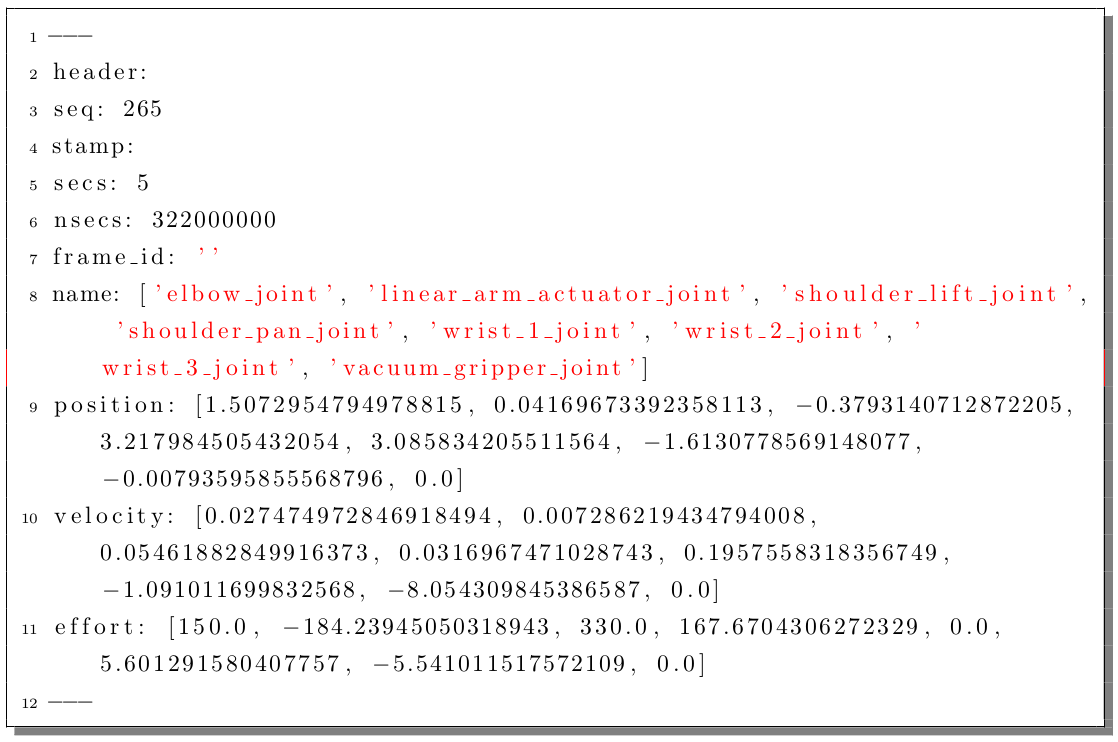
\includegraphics[width=0.9\textwidth]{mensajestate.png}
		\end{figure}
	\end{center}
\end{hslide}

\begin{hslide}
	\slsubsect{Mensaje de orden}
	\begin{center}
		\begin{figure}
			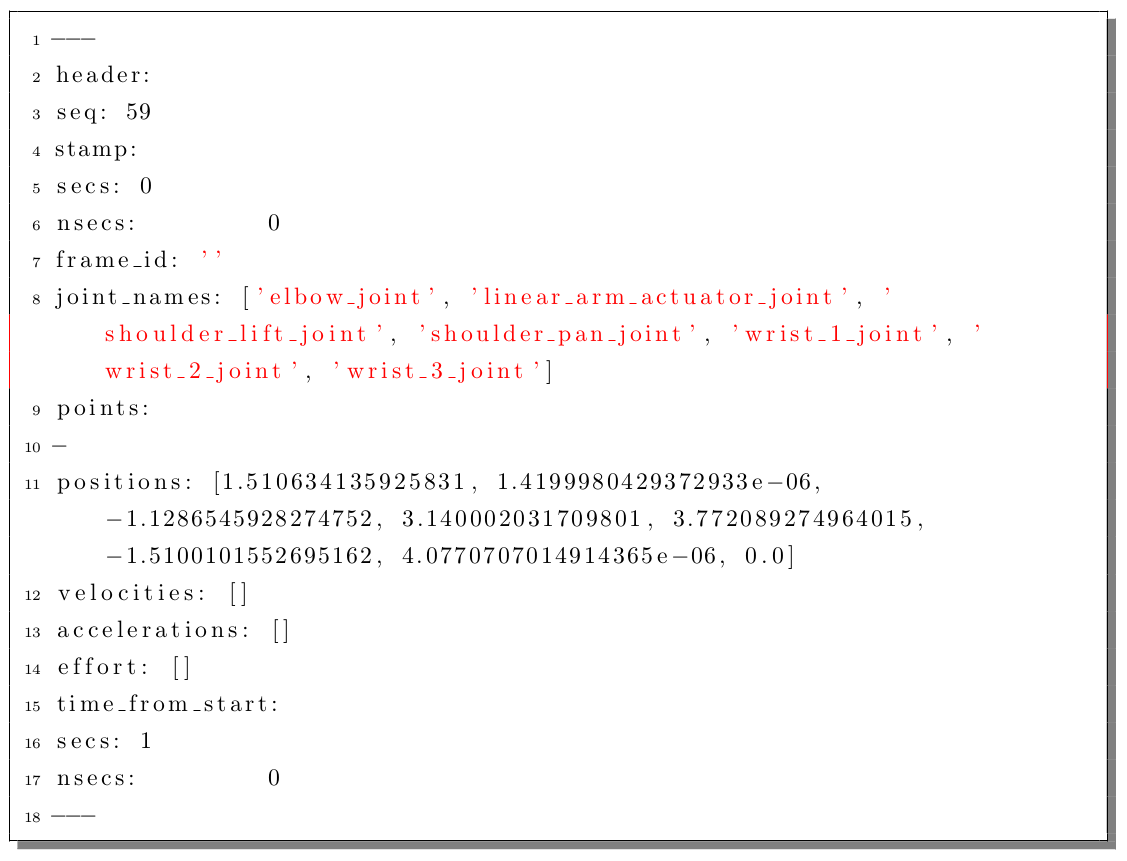
\includegraphics[width=0.8\textwidth]{mensajecommand.png}
		\end{figure}
	\end{center}
\end{hslide}

\begin{hslide}
	\slsubsect{Teleoperador}
	\begin{itemize}
		\item \textbf{Bajo nivel}: Actúa directamente sobre las articulaciones.
		\item \textbf{Interfaz gráfica}: Construida con Qt, manejo intuitivo.
		\item \textbf{Python}: Programado en Python, compatible con ROS y JdeRobot.
	\end{itemize}
	\begin{center}
		\begin{figure}
			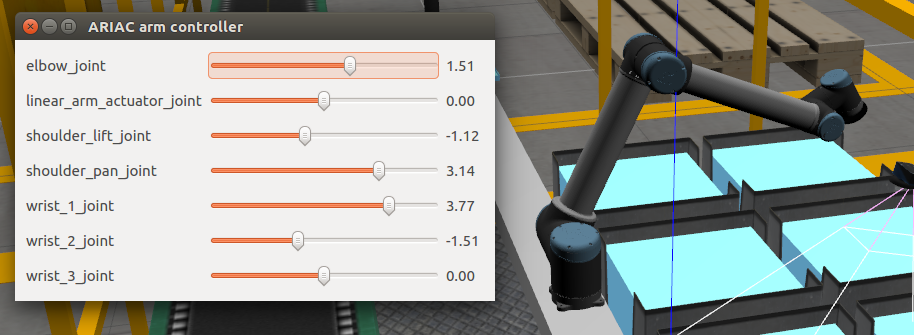
\includegraphics[width=\textwidth]{mando.png}
		\end{figure}
	\end{center}
\end{hslide}

%%---------------------------------------------------------------
\begin{hslide}
	\slsect{Conclusiones}
	\begin{itemize}
		\item \textbf{Objetivo cumplido}: Ampliar y mejorar la colección de prácticas de JdeRobot-Academy.
		\begin{itemize}
			\item Mundo de Gazebo con el Circuito de Mónaco realista.
			\item Teleoperador para brazo robótico
		\end{itemize}
		\item Preparado para las últimas versiones de JdeRobot (5.5), Gazebo (7) y ROS (Kinetic).
	\end{itemize}
	\vspace{0.5cm}
	Trabajos futuros:
	\begin{itemize}
		\item Mejora del diseño del Fórmula 1.
		\item Uso de planificadores de movimiento articulado.
		\item Desarrollo de práctica \textit{pick\&place}.
	\end{itemize}
\end{hslide}


\begin{hslide}
	\slsect{Enlaces}
	\begin{itemize}
		\item Mediawiki: \url{http://jderobot.org/Avillamil-tfg}
		\item Repositorio:
		
		\url{https://github.com/RoboticsURJC-students/2016-tfg-Alvaro-Villamil}
	\end{itemize}
\end{hslide}







\end{document}
